% ******************************* PhD Thesis Template **************************
% Please have a look at the README.md file for info on how to use the template

\documentclass[a4paper,12pt,times,numbered,print,index]{Classes/PhDThesisPSnPDF}


% ******************************************************************************
% ******************************* Class Options ********************************
% *********************** See README for more details **************************
% ******************************************************************************

% `a4paper'(The University of Cambridge PhD thesis guidelines recommends a page
% size a4 - default option) or `a5paper': A5 Paper size is also allowed as per
% the Cambridge University Engineering Deparment guidelines for PhD thesis
%
% `11pt' or `12pt'(default): Font Size 10pt is NOT recommended by the University
% guidelines
%
% `oneside' or `twoside'(default): Printing double side (twoside) or single
% side.
%
% `print': Use `print' for print version with appropriate margins and page
% layout. Leaving the options field blank will activate Online version.
%
% `index': For index at the end of the thesis
%
% `draftclassic': For draft mode without loading any images (same as draft in book)
%
% `draft': Special draft mode with line numbers, images, and water mark with
% timestamp and custom text. Position of the text can also be modified.
%
% `abstract': To generate only the title page and abstract page with
% dissertation title and name, to submit to the Student Registry
%
% `chapter`: This option enables only the specified chapter and it's references
%  Useful for review and corrections.
%
% ************************* Custom Page Margins ********************************
%
% `custommargin`: Use `custommargin' in options to activate custom page margins,
% which can be defined in the preamble.tex. Custom margin will override
% print/online margin setup.
%
% *********************** Choosing the Fonts in Class Options ******************
%
% `times' : Times font with math support. (The Cambridge University guidelines
% recommend using times)
%
% `fourier': Utopia Font with Fourier Math font (Font has to be installed)
%            It's a free font.
%
% `customfont': Use `customfont' option in the document class and load the
% package in the preamble.tex
%
% default or leave empty: `Latin Modern' font will be loaded.
%
% ********************** Choosing the Bibliography style ***********************
%
% `authoryear': For author-year citation eg., Krishna (2013)
%
% `numbered': (Default Option) For numbered and sorted citation e.g., [1,5,2]
%
% `custombib': Define your own bibliography style in the `preamble.tex' file.
%              `\RequirePackage[square, sort, numbers, authoryear]{natbib}'.
%              This can be also used to load biblatex instead of natbib
%              (See Preamble)
%
% **************************** Choosing the Page Style *************************
%
% `default (leave empty)': For Page Numbers in Header (Left Even, Right Odd) and
% Chapter Name in Header (Right Even) and Section Name (Left Odd). Blank Footer.
%
% `PageStyleI': Chapter Name next & Page Number on Even Side (Left Even).
% Section Name & Page Number in Header on Odd Side (Right Odd). Footer is empty.
%
% `PageStyleII': Chapter Name on Even Side (Left Even) in Header. Section Number
% and Section Name in Header on Odd Side (Right Odd). Page numbering in footer


% ********************************** Preamble **********************************
% Preamble: Contains packages and user-defined commands and settings
% ******************************************************************************
% ****************************** Custom Margin *********************************

% Add `custommargin' in the document class options to use this section
% Set {innerside margin / outerside margin / topmargin / bottom margin}  and
% other page dimensions
\ifsetCustomMargin
  \RequirePackage[left=37mm,right=30mm,top=35mm,bottom=30mm]{geometry}
  \setFancyHdr % To apply fancy header after geometry package is loaded
\fi

% Add spaces between paragraphs
%\setlength{\parskip}{0.5em}
% Ragged bottom avoids extra whitespaces between paragraphs
\raggedbottom
% To remove the excess top spacing for enumeration, list and description
%\usepackage{enumitem}
%\setlist[enumerate,itemize,description]{topsep=0em}

% *****************************************************************************
% ******************* Fonts (like different typewriter fonts etc.)*************

% Add `customfont' in the document class option to use this section

\ifsetCustomFont
  % Set your custom font here and use `customfont' in options. Leave empty to
  % load computer modern font (default LaTeX font).
  %\RequirePackage{helvet}

  % For use with XeLaTeX
  %  \setmainfont[
  %    Path              = ./libertine/opentype/,
  %    Extension         = .otf,
  %    UprightFont = LinLibertine_R,
  %    BoldFont = LinLibertine_RZ, % Linux Libertine O Regular Semibold
  %    ItalicFont = LinLibertine_RI,
  %    BoldItalicFont = LinLibertine_RZI, % Linux Libertine O Regular Semibold Italic
  %  ]
  %  {libertine}
  %  % load font from system font
  %  \newfontfamily\libertinesystemfont{Linux Libertine O}
\fi

% *****************************************************************************
% **************************** Custom Packages ********************************

% ************************* Algorithms and Pseudocode **************************

%\usepackage{algpseudocode}


% ********************Captions and Hyperreferencing / URL **********************

% Captions: This makes captions of figures use a boldfaced small font.
%\RequirePackage[small,bf]{caption}

\RequirePackage[labelsep=space,tableposition=top]{caption}
\renewcommand{\figurename}{Fig.} %to support older versions of captions.sty


% *************************** Graphics and figures *****************************

%\usepackage{rotating}
%\usepackage{wrapfig}

% Uncomment the following two lines to force Latex to place the figure.
% Use [H] when including graphics. Note 'H' instead of 'h'
%\usepackage{float}
%\restylefloat{figure}

% Subcaption package is also available in the sty folder you can use that by
% uncommenting the following line
% This is for people stuck with older versions of texlive
%\usepackage{sty/caption/subcaption}
\usepackage{subcaption}

% ********************************** Tables ************************************
\usepackage{booktabs} % For professional looking tables
\usepackage{multirow}

%\usepackage{multicol}
%\usepackage{longtable}
%\usepackage{tabularx}


% *********************************** SI Units *********************************
\usepackage{siunitx} % use this package module for SI units


% ******************************* Line Spacing *********************************

% Choose linespacing as appropriate. Default is one-half line spacing as per the
% University guidelines

% \doublespacing
% \onehalfspacing
% \singlespacing


% ************************ Formatting / Footnote *******************************

% Don't break enumeration (etc.) across pages in an ugly manner (default 10000)
%\clubpenalty=500
%\widowpenalty=500

%\usepackage[perpage]{footmisc} %Range of footnote options


% *****************************************************************************
% *************************** Bibliography  and References ********************

%\usepackage{cleveref} %Referencing without need to explicitly state fig /table

% Add `custombib' in the document class option to use this section
\ifuseCustomBib
   \RequirePackage[square, sort, numbers, authoryear]{natbib} % CustomBib

% If you would like to use biblatex for your reference management, as opposed to the default `natbibpackage` pass the option `custombib` in the document class. Comment out the previous line to make sure you don't load the natbib package. Uncomment the following lines and specify the location of references.bib file

%\RequirePackage[backend=biber, style=numeric-comp, citestyle=numeric, sorting=nty, natbib=true]{biblatex}
%\bibliography{References/references} %Location of references.bib only for biblatex

\fi

% changes the default name `Bibliography` -> `References'
\renewcommand{\bibname}{References}


% ******************************** Roman Pages *********************************
% The romanpages environment set the page numbering to lowercase roman one
% for the contents and figures lists. It also resets
% page-numbering for the remainder of the dissertation (arabic, starting at 1).

\newenvironment{romanpages}{
  \setcounter{page}{1}
  \renewcommand{\thepage}{\roman{page}}}
{\newpage\renewcommand{\thepage}{\arabic{page}}}


% ******************************************************************************
% ************************* User Defined Commands ******************************
% ******************************************************************************

% *********** To change the name of Table of Contents / LOF and LOT ************

%\renewcommand{\contentsname}{My Table of Contents}
%\renewcommand{\listfigurename}{My List of Figures}
%\renewcommand{\listtablename}{My List of Tables}


% ********************** TOC depth and numbering depth *************************

\setcounter{secnumdepth}{2}
\setcounter{tocdepth}{2}


% ******************************* Nomenclature *********************************

% To change the name of the Nomenclature section, uncomment the following line

%\renewcommand{\nomname}{Symbols}


% ********************************* Appendix ***********************************

% The default value of both \appendixtocname and \appendixpagename is `Appendices'. These names can all be changed via:

%\renewcommand{\appendixtocname}{List of appendices}
%\renewcommand{\appendixname}{Appndx}

% *********************** Configure Draft Mode **********************************

% Uncomment to disable figures in `draftmode'
%\setkeys{Gin}{draft=true}  % set draft to false to enable figures in `draft'

% These options are active only during the draft mode
% Default text is "Draft"
%\SetDraftText{DRAFT}

% Default Watermark location is top. Location (top/bottom)
%\SetDraftWMPosition{bottom}

% Draft Version - default is v1.0
%\SetDraftVersion{v1.1}

% Draft Text grayscale value (should be between 0-black and 1-white)
% Default value is 0.75
%\SetDraftGrayScale{0.8}


% ******************************** Todo Notes **********************************
%% Uncomment the following lines to have todonotes.

%\ifsetDraft
%	\usepackage[colorinlistoftodos]{todonotes}
%	\newcommand{\mynote}[1]{\todo[author=kks32,size=\small,inline,color=green!40]{#1}}
%\else
%	\newcommand{\mynote}[1]{}
%	\newcommand{\listoftodos}{}
%\fi

% Example todo: \mynote{Hey! I have a note}


\usepackage{algorithm}
\usepackage[noend]{algpseudocode}

\makeatletter
\def\BState{\State\hskip-\ALG@thistlm}
\makeatother

\usepackage{graphicx, ifpdf, array, xstring, amsfonts, amsmath,multirow,rotating, nameref}
\newcommand{\currHeading}{@currentlabelname}

\newcommand{\kwTransaction}[2]{\textit{#1transaction#2}}
\newcommand{\kwBlock}[1]{\textit{block#1}}
\newcommand{\kwInput}[1]{\textit{input#1}}
\newcommand{\kwOutput}[1]{\textit{output#1}}
\newcommand{\kwCoin}[1]{\textit{coin#1}}
%\newcommand{\mathIn}[1]{$#1$}
%\newcommand{\varCoin}{c}
%\newcommand{\varSN}{S}
%\newcommand{\varCoinR}{r}

\newcommand{\varPComm}{p_{comm}}
\newcommand{\varQComm}{q_{comm}}
\newcommand{\varGComm}{g_{comm}}
\newcommand{\varHComm}{h_{comm}}
\newcommand{\varChallenge}{\mathcal{C}}
\newcommand{\varAccPoKCoinComm}{\mathfrak{C}_c}
\newcommand{\varAccPoKProofComm}[1]{C_#1}
\newcommand{\varAccPoKPComm}{\mathfrak{p}}
\newcommand{\varAccPoKQComm}{\mathfrak{q}}
\newcommand{\varAccPoKGComm}{\mathfrak{g}}
\newcommand{\varAccPoKHComm}{\mathfrak{h}}
\newcommand{\varAccPoKPProof}{p_{QRN}}
\newcommand{\varAccPoKQProof}{q_{QRN}}
\newcommand{\varAccPoKGProof}{g_{QRN}}
\newcommand{\varAccPoKHProof}{h_{QRN}}
\newcommand{\varPSok}{p_{SoK}}
\newcommand{\varQSok}{q_{SoK}}
\newcommand{\varGSok}{g_{SoK}}
\newcommand{\varHSok}{h_{SoK}}
\newcommand{\varLambdaSec}{\lambda_{zkp}}

\newcommand{\eqnAccum}[2]{Accumulate((N,\allowbreak#1),\allowbreak#2)\rightarrow A}
\newcommand{\eqnGenWit}[2]{GenWtiness((N,u),#1,C)\rightarrow #2}
\newcommand{\eqnAccVer}[1]{AccVerify((N,\allowbreak u),A,#1,w)\rightarrow \{0,1\}}
\newcommand{\eqnAccPoK}{NIZKPoK\{(c,w):AccVerify((N,u),A,c,w)=1 \wedge c \in [\mathfrak{A},\mathfrak{B}]\}}
\newcommand{\eqnAccPoKActual}{
	
	\[ NIZKPoK(c,\beta,\gamma,\delta,\varepsilon,\zeta,\varphi,\psi,\eta,\sigma,\xi): \{ \]
	
	\[ \varAccPoKCoinComm=\varAccPoKGComm^c \varAccPoKHComm^\varphi \wedge
	\varAccPoKGComm=(\varAccPoKCoinComm/\varAccPoKGComm)^\gamma \varAccPoKHComm^\psi \wedge 
	\varAccPoKGComm=(\varAccPoKGComm\varAccPoKCoinComm)^\sigma \varAccPoKHComm^\xi \wedge 
	\]
	
	\[
	\varAccPoKProofComm{r}=\varAccPoKGProof^\varepsilon \varAccPoKHProof^\zeta \wedge 
	\varAccPoKProofComm{c}=\varAccPoKGProof^c \varAccPoKHProof^\eta \wedge 
	A=\varAccPoKProofComm{w}^c (1/\varAccPoKHProof)^\beta \wedge 
	\]
	
	\[
	1=\varAccPoKProofComm{r}^c (1/\varAccPoKHProof)^\delta (1/\varAccPoKGProof)^\beta \wedge
	c \in [\mathfrak{A},\mathfrak{B}]\}
	\]
}
\newcommand{\eqnSNSoK}{ZKSoK[m]\{(c,r):c=\varGComm^S\varHComm^r\}}
\newcommand{\eqnSNSoKActual}{ZKSoK[m]\{(c,r,z):y=\expSoKCoinComm{\expPedCommCoin}\}}
\newcommand{\eqnCommPoK}{NIZKPoK\{(c,\varphi,z):\varAccPoKCoinComm=\varAccPoKGComm^{c}\varAccPoKHComm^{\varphi} \wedge y=\expSoKCoinComm{c}\}}

\newcommand{\expIntGroup}[1]{\mathbb{Z}_{#1}}
\newcommand{\expMulGroup}[1]{\mathbb{Z}_{#1}^{*}}
\newcommand{\expPedCommCoin}{\varGComm^{S}\varHComm^{r}}
\newcommand{\expSoKCoinComm}[1]{\varGSok^{#1}\varHSok^{z}}
\newcommand{\expOneToN}[2]{#1_1,\cdots,#1_#2}
\newcommand{\expAFrak}{\mathfrak{A}=-\varPComm2^{k'+k''+2}}
\newcommand{\expBFrak}{\mathfrak{B}=\varPComm2^{k'+k''+2}}
\newcommand{\expConcatAccPoK}{
	\varAccPoKCoinComm \|
	\varAccPoKProofComm{c} \|
	\varAccPoKProofComm{w} \|
	\varAccPoKProofComm{r} \|
	\varAccPoKGComm \|
	\varAccPoKHComm \|
	\varAccPoKGProof \|
	\varAccPoKHProof \|
	t_i \cdots
}
\newcommand{\expConcatSNSoK}{
	y \|
	S \|
	\varGSok \|
	\varHSok \|
	t_1 \|
	\cdots \|
	t_{\varLambdaSec} \|
	m
}
\newcommand{\expConcatPrimeSNSoK}{
	y \|
	S \|
	\varGSok \|
	\varHSok \|
	t'_1 \|
	\cdots \|
	t'_{\varLambdaSec} \|
	m
}
\newcommand{\expConcatCommPoK}{
	\varAccPoKCoinComm \|
	y \|
	t_1 \|
	t_2 \|
	\varAccPoKGComm \|
	\varAccPoKHComm \|
	\varGSok \|
	\varHSok
}
\newcommand{\expConcatSNSoKImproved}{
	y \|
	S \|
	\varGSok \|
	\varHSok \|
	t \|
	m
}
\newcommand{\expConcatAccPoKFull}{
	\varAccPoKCoinComm \| \allowbreak
	\varAccPoKProofComm{c} \| \allowbreak
	\varAccPoKProofComm{w} \| \allowbreak
	\varAccPoKProofComm{r} \| \allowbreak
	\varAccPoKGComm \| \allowbreak
	\varAccPoKHComm \| \allowbreak
	\varAccPoKGProof \| \allowbreak
	\varAccPoKHProof \| \allowbreak
	\mathfrak{t}_1 \| \allowbreak
	\mathfrak{t}_2 \| \allowbreak
	\mathfrak{t}_3 \| \allowbreak
	t_1 \| \allowbreak
	t_2 \| \allowbreak
	t_3 \| \allowbreak
	t_4
}
\newcommand{\expConcatAccPoKImproved}{
	\varAccPoKCoinComm \| \allowbreak
	\varAccPoKProofComm{c} \| \allowbreak
	\varAccPoKProofComm{w} \| \allowbreak
	\varAccPoKProofComm{r} \| \allowbreak
	\varAccPoKGComm \| \allowbreak
	\varAccPoKHComm \| \allowbreak
	\varAccPoKGProof \| \allowbreak
	\varAccPoKHProof \| \allowbreak
	\mathfrak{t}'_1 \| \allowbreak
	\mathfrak{t}'_2 \| \allowbreak
	\mathfrak{t}'_3 \| \allowbreak
	t'_1 \| \allowbreak
	t'_2 \| \allowbreak
	t'_3 \| \allowbreak
	t'_4
}


% ************************ Thesis Information & Meta-data **********************
% Thesis title and author information, refernce file for biblatex
% ************************ Thesis Information & Meta-data **********************
%% The title of the thesis
\title{Making Privacy in Digital Currency Practical by Improving the Efficiency of the Zerocoin Protocol}
%\texorpdfstring is used for PDF metadata. Usage:
%\texorpdfstring{LaTeX_Version}{PDF Version (non-latex)} eg.,
%\texorpdfstring{$sigma$}{sigma}

%% Subtitle (Optional)
%\subtitle{Using the CUED template}

%% The full name of the author
\author{Shao Fei}

%% Department (eg. Department of Engineering, Maths, Physics)
\dept{Department of Electrical and Computer Engineering}

%% University and Crest
\university{National University of Singapore}
% Crest minimum should be 30mm.
\crest{
\includegraphics[width=0.2\textwidth]{NUS-fullcolorlogo_v}}
%% Use this crest, if you are using the college crest
%% Crest long miminum should be 65mm
%\crest{\includegraphics[width=0.45\textwidth]{University_Crest_Long}}

%% College shield [optional] 
% Crest minimum should be 30mm.
%\collegeshield{\includegraphics[width=0.2\textwidth]{CollegeShields/Kings}}


%% Supervisor (optional)
\supervisor{Prof. Bharadwaj Veeravalli}
%% Supervisor Role (optional) - Supervisor (default) or advisor
%\supervisorrole{Advisor: }

%% Advisor (optional)
\advisor{Jestine Paul}
%% Advisor Role (optional) - Advisor (default) or leave empty
%\advisorrole{Advisor: }


%% You can redefine the submission text:
% Default as per the University guidelines:
% ``This dissertation is submitted for the degree of''
\renewcommand{\submissiontext}{This interim report is submitted for the degree of}

%% Full title of the Degree
\degreetitle{B.Eng (Computer Engineering)}

%% College affiliation (optional)
%\college{King's College}

%% Submission date
% Default is set as {\monthname[\the\month]\space\the\year}
%\degreedate{September 2014} 

%% Meta information
\subject{LaTeX} \keywords{{LaTeX} {PhD Thesis} {Engineering} {University of
Cambridge}}

% ***************************** Abstract Separate ******************************
% To printout only the titlepage and the abstract with the PhD title and the
% author name for submission to the Student Registry, use the `abstract' option in
% the document class.

\ifdefineAbstract
 \pagestyle{empty}
 \includeonly{Declaration/declaration, Abstract/abstract}
\fi

% ***************************** Chapter Mode ***********************************
% The chapter mode allows user to only print particular chapters with references
% Title, Contents, Frontmatter are disabled by default
% Useful option to review a particular chapter or to send it to supervisior.
% To use choose `chapter' option in the document class

\ifdefineChapter
 \includeonly{Chapter3/chapter3}
\fi

% ******************************** Front Matter ********************************
\begin{document}

\frontmatter

\begin{titlepage}
  \maketitle
\end{titlepage}


%% ******************************* Thesis Dedidcation ********************************

\begin{dedication} 

I would like to dedicate this thesis to my loving parents \dots

\end{dedication}
%% ******************************* Thesis Declaration ***************************

\begin{declaration}

I hereby declare that except where specific reference is made to the work of 
others, the contents of this dissertation are original and have not been 
submitted in whole or in part for consideration for any other degree or 
qualification in this, or any other university. This dissertation is my own 
work and contains nothing which is the outcome of work done in collaboration 
with others, except as specified in the text and Acknowledgements. This 
dissertation contains fewer than 65,000 words including appendices, 
bibliography, footnotes, tables and equations and has fewer than 150 figures.

% Author and date will be inserted automatically from thesis.tex \author \degreedate

\end{declaration}
%% ************************** Thesis Acknowledgements **************************

\begin{acknowledgements}      


And I would like to acknowledge ...


\end{acknowledgements}

% ************************** Thesis Abstract *****************************
% Use `abstract' as an option in the document class to print only the titlepage and the abstract.
\begin{abstract}
	Digital currencies such as Bitcoin provide some level of privacy because users can use multiple arbitrary identities to make transactions. However the caveat is that transaction records are public and unencrypted, and thus there are various ways to de-anonymise users. This research uses Bitcoin as a starting point to analyse the issues surrounding privacy in digital currencies and explores the various ways to overcome these issues. Zerocoin, an anonymous digital currency protocol based on Non-Interactive Zero-knowledge proofs, shows promise and is examined in detail. The main performance drawbacks in Zerocoin are the large computational and storage requirements for its proofs. If these problems are addressed, Zerocoin can be a commercially viable anonymous digital currency. This research attempts to reduce the performance overheads in Zerocoin by modifying the Accumulator Proof of Knowledge (AccPoK) and Serial Number Signature of Knowledge (SNSoK) in the protocol. The proposed SNSoK is a modification of the proof for a committed value in a Pedersen commitment, and is smaller and faster that the original SNSoK by about 40 times and 80 times respectively. The proposed AccPoK employs an optimisation technique that is used in the original SNSoK, but its performance has not been tested. Going forward, this research plans to continue enhancing the proposed improvements and simulate a Zerocoin network to test them on a network level. If time permits, this research will also explore ways to enhance the functionality aspects of Zerocoin.
  
\end{abstract}


% *********************** Adding TOC and List of Figures ***********************

\tableofcontents

\listoffigures

\listoftables

% \printnomenclature[space] space can be set as 2em between symbol and description
%\printnomenclature[3em]


% ******************************** Main Matter *********************************
\mainmatter
\chapter*{Introduction}
Privacy is a major theme in any financial transaction system. While traditional banking systems offer privacy by keeping transaction records private, the centralised records can be exposed either maliciously or under the order of authorities. Since banks keep the real identities of transaction owners for accountability, privacy is completely destroyed when the records are exposed. Bitcoin as a digital currency system addresses some of the privacy problems of traditional banking by providing a level of “pseudonymity” through the use of arbitrary public key addresses as identities during payments (\S\ref{sec:1-Pseudonymity of Bitcoin}). This has partly driven the immense popularity of Bitcoin, which has a market capitalisation of USD\$10 billion and daily transactions volume of USD\$50 million as of October 2016\footnote{Based on statistics from https://coinmarketcap.com/}.

However due to the decentralised nature of Bitcoin, Bitcoin transaction records are unencrypted and publicly available. Even though transactions are executed with cryptic public key addresses, there are many techniques to de-anonymise Bitcoin transactions (\S\ref{sec:1-Ways to De-anonymise Bitcoin}). In order to preserve the privacy of Bitcoin, different innovations has been developed. Methods such Mixing can be easily integrated with Bitcoin, while others require separate digital currency systems, referred to as Altcoins, to be implemented (\S\ref{ch:Methods to Improve Privacy in Digital Currencies}).

One Altcoin, Zerocoin, which makes use of Non-interactive Zero Knowledge (NIZK) proofs to create and validate anonymous transactions, is identified as the subject of research due to its theoretical soundness and practical potential (\S\ref{sec:2-Selection Zerocoin as the Subject of Research}). This research attempts to address the computational and storage inefficiencies in Zerocoin (\S\ref{sec:2-Zerocoin Drawbacks}) so that it can be a viable substitute to the current Bitcoin system. This will be mainly done by modifying the NIZK proofs algorithms and related data structures (\S\ref{sec:3-NIZK Proofs in Zerocoin}) in the Zerocoin protocol. The proposed improvements will be benchmarked against the original Zerocoin protocol in terms of privacy preservation and computational performance (\S\ref{sec:4-Performance Metrics and Benchmarks}). The objective of the research is to achieve a considerable improvement in computational performance without significant compromise in privacy preservation.

At this point, this research has examined the theoretical basis and the construction of Zerocoin (\S\ref{ch:Analysis of Zerocoin}). The source code of the Zerocoin protocol developed by its creators has also been analysed and some areas for improvement have been identified (\S\ref{sec:3-Performance of Zerocoin and Areas for Improvement}). Improvements have also been proposed and tested by modifying the Zerocoin source code (\S\ref{ch:Contribution 1: A more Efficient Serial Number Signature of Knowledge} and \S\ref{ch:Contribution 2: A Smaller Accumulator Proof of Knowledge}). This research plans to continue refining the proposed improvements and test their performance on a network level by simulating a peer-to-peer Zerocoin network (\S\ref{sec:4-Performance Metrics and Benchmarks}). 
%*******************************************************************************
%*********************************** First Chapter *****************************
%*******************************************************************************

\ifpdf
\graphicspath{{Chapter1/Figs/}}
\else
\graphicspath{{Chapter1/Figs/}}
\fi

\chapter{Privacy in Bitcoin}  %Title of the First Chapter
\label{ch:Privacy in Bitcoin}
\section{Overview of Bitcoin} %Section - 1.1 
\label{sec:1-Overview of Bitcoin}
To facilitate better understanding of the issues surrounding anonymity in Bitcoin and digital currencies in general, this paper introduces a basic model of Bitcoin. For conciseness, only parts of Bitcoin that relate to anonymity are presented and the other concepts are simplified. The explanations of Bitcoin are adapted from \cite{andreas2014mastering} and \cite{narayanan2016bitcoin}.

As defined by to the creator of Bitcoin Satoshi Nakamoto, Bitcoin is a purely peer-to-peer electronic cash system that allows direct online payments without going through a financial institution \cite{Nakamoto2008}.  When a payer wants to make a payment, he constructs a \kwTransaction{}{} and broadcast it to the Bitcoin peer-to-peer network, where it can be validated by any peer (interchangeably referred to as node) through its digital signature. A simplified data structure for a \kwTransaction{}{} is shown in Fig.~\ref{fig:bitcoin_transactions}:

\begin{figure}[H]
	\begin{center}
		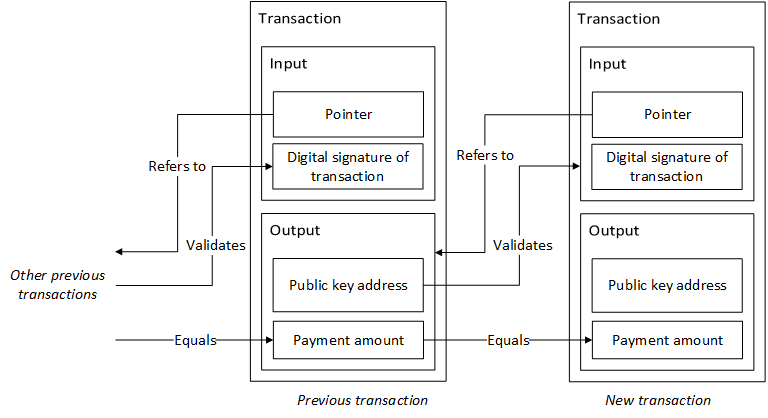
\includegraphics[scale=0.7]{bitcoin-transactions} 
		\caption{Bitcoin \textit{transactions}}
		\label{fig:bitcoin_transactions} 
	\end{center}
\end{figure}

Each \kwTransaction{}{} has a set of \kwOutput{s} which denotes public key addresses (destination of payment) and the payment amounts. For a payment to be valid, the payer must have the funds to make the payment.  The set of \kwInput{s} in a \kwTransaction{}{} denotes the source of funds used in the payment. To denote the payer’s source of funds, an \kwInput{} refers to a previous \kwOutput{} that has been paid to the public key address of the payer. Essentially a payer is using some funds that are previously paid to him/her to pay the payee. In order for the \kwTransaction{}{} to be valid, the payer must indeed own the public keys address that the previous \kwOutput{} has paid to. Nodes in the Bitcoin network validates this by checking whether the digital signature signed by the payer’s private key in the \kwInput{} is valid under the public key address in the previous \kwOutput{} referred to by the \kwInput{}. If the digital signature is valid, it means that the payer knows the private key that corresponds to the public key address that the previous \kwOutput{} has paid to, and he indeed owns the public key address. The example above shows the case where there is only one \kwInput{} and one \kwOutput{} in a transaction, but a \kwTransaction{}{} can have multiple \kwInput{s} and \kwOutput{s}. In such cases, the payer is combining sources of funds from multiple public key addresses and paying them to multiple payment addresses. At this point, it can be noted that a user can own multiple public key addresses which is achieved by simply creating them.

In addition to proof of ownership of funds, the amounts referenced by in the \kwInput{} and the amount stated in the \kwOutput{} of a \kwTransaction{}{} must also be equal. For cases where there are multiple \kwInput{s} and \kwOutput{s} in a transaction, the total amount in the previous \kwOutput{s} referenced by the \kwInput{s} must equal to the total amount stated by the \kwOutput{s}. Essentially, this means that the source of payment must be in the correct amount to fulfil the payment. Another point note is that a previous \kwOutput{} referenced by an \kwInput{} must be consumed in full, which means that the funds in the previous \kwOutput{} cannot be broken down to make a payment of an exact amount. Change is given back to the payer by creating an additional \kwOutput{} in the \kwTransaction{}{} that pays back the excess amount to one of the payer’s public key address. This mechanism ensures that the \kwInput{} and \kwOutput{} amounts of a \kwTransaction{}{} always tally. Lastly, to prevent double spending, the previous \kwOutput{} that is referenced by the \kwInput{} must not be already referenced by the \kwInput{} of another \kwTransaction{}{}.

Once a node has performed all the above checks and validated a transaction, it forwards the \kwTransaction{}{} to its neighbours who carry on the process. If the node who receives the \kwTransaction{}{} happens to be a miner node, it combines the \kwTransaction{}{} with other \kwTransaction{}{s} to form a block, and attempts to publish the \kwBlock{} to the Blockchain through the consensus protocol. The new \kwBlock{} that passes the consensus protocol is accepted by all nodes and extends the Blockchain by pointing to the latest \kwBlock{} in the Blockchain. A simplified example illustrating the relationships between \kwBlock{s} and \kwTransaction{}{s} in the Blockchain is shown in Fig.~\ref{fig:bitcoin_blockchain}.

\begin{figure}[H]
	\begin{center}
		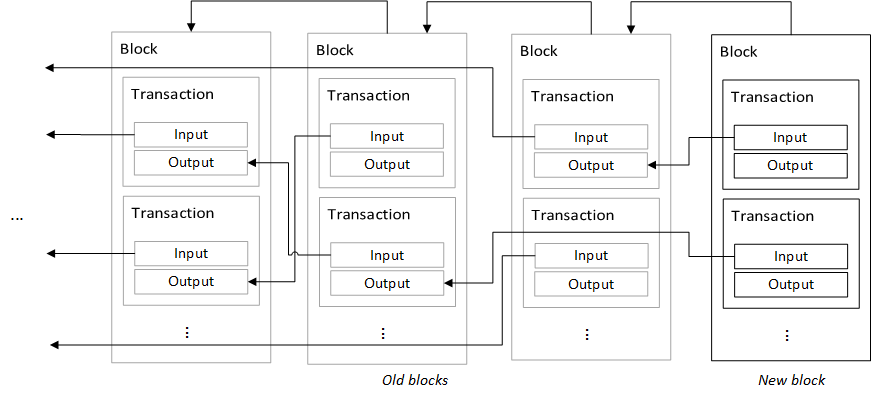
\includegraphics[scale=0.65]{bitcoin-blockchain} 
		\caption{\textit{blocks} and \textit{transactions} in the Blockchain}
		\label{fig:bitcoin_blockchain} 
	\end{center}
\end{figure}

As seen, the Blockchain contains nothing but chains of transfers of ownership of funds from the public key address in one \kwOutput{} to the public key address in another \kwOutput{} across different \kwBlock{s}. Those \kwOutput{s} that are not referred to by any \kwInput{} represent unspent funds, and can be referenced to by a new transaction.

Once a \kwTransaction{}{} has made it to the Blockchain for some while, the payment is considered confirmed.  The append-only property of the Blockchain prevents confirmed \kwTransaction{}{} from being tampered, while the public nature of the Blockchain allows anyone to check for the validity of a \kwTransaction{}{}.These features ensures that Bitcoin payments are secure. 

\section{Pseudonymity of Bitcoin}
\label{sec:1-Pseudonymity of Bitcoin}
\textbf{\textit{Pseudonymity}} refers to the case of a user using an identity that is not his/her real identity \cite{narayanan2016bitcoin}. Bitcoin achieves pseudonymity as payments made with public key addresses instead of real world identities. These addresses are generated randomly, and a user can generate as many public key addresses as he wants to further hide his/her identity. Hence it is impossible to tell who a public key address belongs to given only the information of the public key address. However pseudonymity alone in Bitcoin does not achieve privacy as public key addresses can still be linked to real world identities given other information (\S\ref{sec:1-Ways to De-anonymise Bitcoin}). Due to the public nature of the Blockchain, once a real world identity is linked to a public key address, all the \kwTransaction{}{s} in the past, present and future using that address can be linked to that real world identity.

\section{Definition of Anonymity and Anonymity Set}
\label{sec:1-Definition of Anonymity and Anonymity Set}
To achieve privacy in Bitcoin, the anonymity property needs to be satisfied. Anonymity in the context of Bitcoin requires pseudonymity and unlinkability \cite{narayanan2016bitcoin}. \textbf{\textit{Unlinkability}} refers to the case that it is hard to:

\begin{enumerate}
	\item Link different public key addresses of the same user
	\item Link different \kwTransaction{}{s} made by the same user
	\item Link a payer to the payee 
\end{enumerate}

If the above properties are satisfied, Bitcoin and digital currency systems in general can be truly anonymous and \kwTransaction{}{s} can be fully private. 

Another term that is relevant to anonymity is the \textbf{\textit{anonymity set}} \cite{narayanan2016bitcoin}. An anonymity set in Bitcoin is the set of \kwTransaction{}{s} in which an adversary cannot distinguish a particular \kwTransaction{}{} from. In other words, even if an adversary knows that a \kwTransaction{}{} is linked to a particular user, he cannot identify which \kwTransaction{}{} it is if that \kwTransaction{}{} is in its anonymity set. An anonymity set containing one \kwTransaction{}{} essentially implies no anonymity, while an anonymity set containing all the \kwTransaction{}{s} on the Blockchain implies full anonymity. Hence the size of the anonymity set in a protocol can be used to measure its level of anonymity.

\section{Ways to De-anonymise Bitcoin}
\label{sec:1-Ways to De-anonymise Bitcoin}
\subsection{Linking Payers to Payee}
\label{sec:1-Linking Payers to Payee}
Given the properties of anonymity, it can be seen that Bitcoin is not anonymous. The current Bitcoin protocol clearly violates the property that it should be hard to link a payer to the payee. The \kwInput{} of a \kwTransaction{}{} provides the link to the payer’s public key address, while the \kwOutput{} of a \kwTransaction{}{} states the payee’s public key address. For cases of direct payments without the use of an intermediary, anyone can easily tell the link between the payer and the payee since all \kwTransaction{}{s} are public on the Blockchain. 

\subsection{Linking Public Key Addresses and Transactions}
\label{sec:1-Linking Public Key Addresses and Transactions}
The other two anonymity properties apply to cases where users use different public key addresses for payments. These two properties can be violated when the different public key addresses used by the same user are linked together to form a \textbf{\textit{cluster}}. If this is achieved, then the only step left is to associate a real world identity to the cluster to fully de-anonymise the user. 

The first step of forming clusters of addresses can be achieved by inferring joint control of addresses through \textbf{\textit{shared spending}} and \textbf{\textit{shadow addresses}} \cite{Androulaki2013}. This technique is illustrated in Fig.~\ref{fig:bitcoin_cluster}.

\begin{figure}[H]
	\begin{center}
		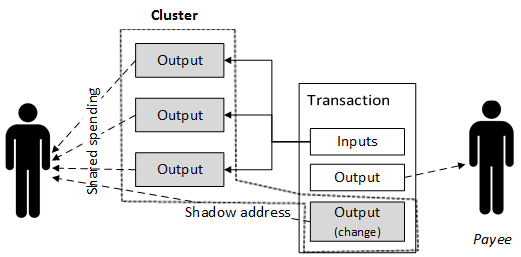
\includegraphics[scale=0.9]{bitcoin-cluster} 
		\caption{Clustering by inferring joint control of addresses}
		\label{fig:bitcoin_cluster} 
	\end{center}
\end{figure}

A \kwTransaction{}{} can contain shared spending by having multiple \kwInput{s} that refer to a different previous \kwOutput{s} (\S\ref{sec:1-Overview of Bitcoin}). One of the main reason for this kind of \kwTransaction{}{} is that the payment amount is too big to be fulfilled by any single \kwOutput{} paid to the payer and the payer has to combine funds from different \kwOutput{s} to make the payment. An adversary can make use of this spending pattern and infer that the public key addresses in the \kwOutput{s} referred to by the \kwInput{s} in a \kwTransaction{}{} belong to the same payer. In addition, a \kwTransaction{}{} often contains an \kwOutput{} that pays back the change to the payer (\S\ref{sec:1-Overview of Bitcoin}). The public key addresses in these \kwOutput{s}. referred to as shadow addresses, are in fact the addresses of payer. Hence an adversary can attempt extract these shadow addresses from a \kwTransaction{}{}.These two techniques can be used to form clusters of public key addresses that belong the same user. In the above example, the \kwOutput{s} in grey form a cluster and the public key addresses in these \kwOutput{s} belong to the Payer. Once clusters have been formed, different clusters can be linked to each other transitively as long as one public key address from each of the different clusters can be linked together. An example of this technique is illustrated in Fig.~\ref{fig:bitcoin_cluster_transitive}.

\begin{figure}[H]
	\begin{center}
		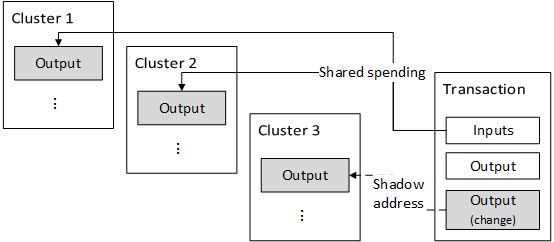
\includegraphics[scale=0.95]{bitcoin-cluster-transitive} 
		\caption{Linking clusters transitively}
		\label{fig:bitcoin_cluster_transitive} 
	\end{center}
\end{figure}

\subsection{Linking Public Key Addresses to Real World Identities}
\label{sec:1-Linking Public Key Addresses to Real World Identities}
After forming clusters of public key addresses that each belongs to a user, the last step is to assign real world identities to the clusters. This can be done by transacting with users who are targets of de-anonymization \cite{Meiklejohn2013}. Given that an adversary knows the real world identity of the user he is transacting with, he can learn one of the public key address of the user. With this one known public key address of the real world identity, a whole cluster containing that public key address can be transitively linked to the identity. Hence an adversary has the ability to attribute a list of public key addresses to a real world identity and de-anonymize the \kwTransaction{}{s} made by that identity.

\subsection{Side Channels Attacks}
\label{sec:1-Side Channels Attacks}
Side channels in Bitcoin refer to the indirect disclosure of information that can aid in the discovery of the real world identity of users. Since all \kwTransaction{}{} information such as payment amounts and timings are publicly available, an adversary can correlate \kwTransaction{}{s} patterns with other publicly available information to match \kwTransaction{}{s} to real identities \cite{narayanan2016bitcoin}. For example if activities on social media are correlated to Bitcoin \kwTransaction{}{s} activity, then social media users (assuming they are using real world identities) can be linked with the \kwTransaction{}{s} that happened during the period when they are active on social media. In addition, similar to clustering \kwTransaction{}{s} by analysing shared spending and shadow addresses, an adversary can also cluster \kwTransaction{}{s} together based on the similarities in the timings and amounts of the \kwTransaction{}{s} \cite{Androulaki2013}. The bottom-line is that as long as \kwTransaction{}{} details are public, there are always ways to make intelligent guesses about the real word identities of public key addresses.   

%*******************************************************************************
%****************************** Second Chapter *********************************
%*******************************************************************************

\ifpdf
\graphicspath{{Chapter2/Figs/}}
\else
\graphicspath{{Chapter2/Figs/}}
\fi

\chapter{Methods to Improve Privacy in Digital Currencies}
\label{ch:Methods to Improve Privacy in Digital Currencies}

The key to achieving anonymity in Bitcoin and any digital currencies is to remove the ability to link a payer to a payee. This immediately satisfies the third property of anonymity that it should be hard to link a payer to a payee. A user can also take advantage of this and make an anonymous payment to himself. Since the public key address that he uses to make the payment cannot be linked to the public key address that he uses to receive the payment, the user can transact with the latter public key address on a clean slate. Hence, the first and second properties of anonymity that it should be hard to link public key addresses and transactions to the same user are also achieved.

\section{Mixing}
\label{sec:2-Mixing}
Mixing is a concept that removes the ability to link a payer to a payee. All methods to improve privacy in digital currencies adopt mixing in one way or another by. The principle of mixing is illustrated in Fig.~\ref{fig:mixing}.

\begin{figure}[H]
	\begin{center}
		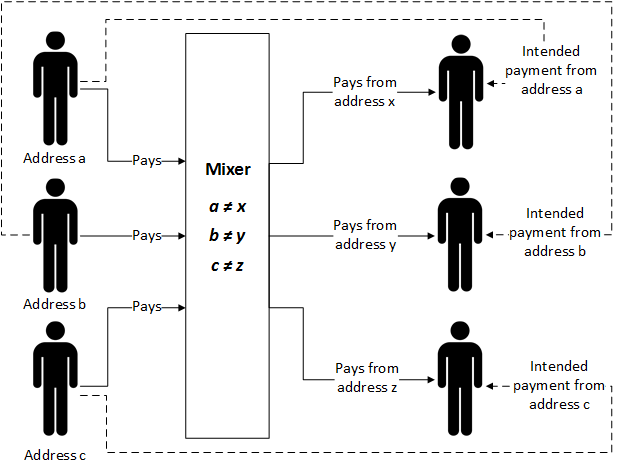
\includegraphics[scale=0.7]{mixing} 
		\caption{Principle of mixing}
		\label{fig:mixing} 
	\end{center}
\end{figure}

To perform mixing, payers make payments via an intermediary called the mixer. The mixer collects payments from payers and pays their intended payee via \kwTransaction{}{s} whose \kwInput{s} do not refer to the public key address of the original payers. In this way observers of the Blockchain are only able to see \kwTransaction{}{s}  from the payers to the mixer and from the mixer to the payee, but cannot tell which payer paid to which payee. The anonymity set in this case is the number of payers participating in the mix, since one only knows that a payer participated in the mixing, but is unable to tell who the payer paid to among the payees that received payments from the mixer.

In order for mixing to work, the amounts that is being transacted via a mixer should be constant for all participants of the mixing protocol \cite{narayanan2016bitcoin}. If different payers pay different amounts to the mixer, and subsequently the mixer pays different amounts to the payees, one can deduce the link between a payer and payee by matching the payment amounts between the payer and the mixer and those between the mixer and the payee. This research has explored several methods of mixing and the issues they face. 

\section{Dedicated Mixing Services and Decentralised Mixing}
\label{sec:2-Dedicated Mixing Services and Decentralised Mixing}
\textbf{Dedicated mixing services} have been commercially implemented in Bitcoin. Services such as Bitcoin Fog and BitLaundry routinely handle 6-digit dollar amounts everyday \cite{Moser2013}. These services act as centralised mixers, where participants make payments to the services and instruct them to transfer the funds to specific address. However dedicated mixing services face some major drawbacks:

\begin{enumerate}
	\item Dedicated mixing services need to keep the transactions records of their users to make fund transfers. Thus privacy is built on the trust that mixing services will not disclose these records. This runs against decentralized principle of Bitcoin and digital currencies in general \cite{narayanan2016bitcoin}.
	\item Since mixers are used for payments, users typically require funds to be transferred immediately to the intended payees. Thus mixers can only work with a limited pool of participants who happen to make payments at the same time. This limits the anonymity set in the mixing protocol, and lowers the level of anonymity in the protocol \cite{narayanan2016bitcoin}.
	\item By exploiting the weakness in point 2 and analysing the mixing patterns adopted by the dedicated mixers, transactions in dedicated mixes can be de-anonymised \cite{Moser2013}. 
\end{enumerate}

\textbf{Decentralised mixing} adopts a peer-to-peer mixing protocol. One such protocol proposed is Coinjoin \cite{Gmaxwell2013}, which gathers payers who wish to participate in mixing to collectively construct a single transaction. Each \kwInput{} in the Coinjoin transaction refers to the funds from each payer, while each \kwOutput{} in the transaction pays to the public key address of each intended payee. The \kwInput{s} and \kwOutput{s} are ordered randomly in the transaction, and an adversary cannot tell which input (payer) corresponds to which output (payee). Here the mixer is the transaction, and the anonymity set is the number of participants in the transaction. Though Coinjoin achieves decentralisation, it still faces the same problem as dedicated mixing services of having a limited anonymity set, as the protocol is carried out with the few payers who want to make payments at the same time. In addition, since a Conjoin transaction is collectively constructed, the protocol faces denial-of-service attacks where an adversary who initially agrees to participate in a Coinjoin transaction refuses to complete his part in the creation of the transaction \cite{narayanan2016bitcoin}.

As seen, Bitcoin mixing techniques that involve the shuffling to payers and payees do not work well in both the centralised and decentralised form. There is also little room for improvement for these protocols as any bigger changes will involve modifications to the Bitcoin protocol that are too costly to implement. Altcoins, on the other hand, have the liberty implement any protocol and thus provide a higher level of anonymity compared to the mixing protocols.

\section{Altcoins: Zerocoin and Zerocash}
\label{sec:2-Altcoins: Zerocoin and Zerocash}
Altcoins are alternative digital currency systems to Bitcoin. The two popular proposed altcoins that provide privacy are Zerocoin and Zerocash. As opposed to the traditional mixers discussed in \S\ref{sec:2-Dedicated Mixing Services and Decentralised Mixing}, Zerocoin and Zerocash provides anonymity using cryptographic guarantees. As these two protocols are very technical, they are only dealt with in concept, with a focus on their capabilities and drawbacks and the reasons why Zerocoin is chosen as the final subject of research. The Zerocoin protocol will then be examined in detail in \S\ref{ch:Analysis of Zerocoin}. Unless otherwise stated, all technical information presented on Zerocoin and Zerocash are obtained from the original Zerocoin \cite{Miers2013} and Zerocash \cite{Ben-Sasson2014} papers.

\subsection{Zerocoin}
\subsubsection{Protocol}
\label{sec:2-Zerocoin Protocol}
Zerocoin extends Bitcoin by incorporating another type of anonymous currency called the “Zerocoin” into the Bitcoin protocol. A comparison between Bitcoin and Zerocoin is shown in Fig.~\ref{fig:zerocoin_overview}.

\begin{figure}[H]
	\begin{center}
		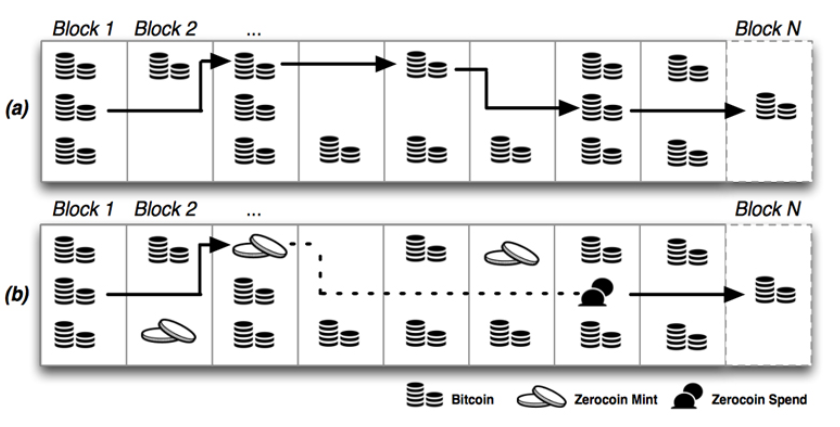
\includegraphics[scale=0.7]{zerocoin-overview} 
		\caption{Comparison between Bitcoin and Zerocoin \cite{Miers2013}}
		\label{fig:zerocoin_overview} 
	\end{center}
\end{figure}

Payments in Bitcoin (a) involves a transfer of funds (Bitcoins) via \kwTransaction{}{s} recorded on the Blockchain. In any block, payments are made using Bitcoins that have been paid to the payer in a previous block (i.e. transaction \kwInput{s} refer to \kwOutput{s} of past \kwTransaction{}{s}).
 
The high level flow of Zerocoin (b) is also similar. In addition to using Bitcoins for payments, users can use their Bitcoins to create an anonymous “Zerocoin” (referred to as \kwCoin{} from now on) via a \kwTransaction{Mint }{}. The exchange rate between Bitcoin and \kwCoin{} is fixed, and thus a Bitcoin always mints the same amount of \kwCoin{}. A \kwCoin{} is a cryptographic commitment $c$ of a serial number $S$ and a secret trapdoor $r$ which are only known to the user who minted the \kwCoin{}. The property of $c$ is that both $S$ and $r$ is needed to obtain the value of $c$, and it is hard to compute the value of $S$ or $r$ from $c$. Like a Bitcoin \kwTransaction{}{}, a \kwTransaction{Mint }{} contains \kwInput{s} that specify the Bitcoins that are used to mint the \kwCoin{}. A \kwTransaction{Mint }{} does not have an \kwOutput{} as it does not make any payment and simply creates a \kwCoin{}. Once the \kwInput{} in a \kwTransaction{Mint }{} is verified to be valid by nodes, it is published on the Blockchain and the minted \kwCoin{} $c$ is added to a public data structure called the \textbf{accumulator} (\S\ref{sec:3-Public Accumulator}). 

The minted \kwCoin{} $c$ can be redeemed and converted to back to Bitcoins later on using a \kwTransaction{Spend }{}. Similar to a Bitcoin \kwTransaction{}{}, the \kwTransaction{Spend }{} contains an \kwInput{} that proves the ownership of $c$, and an \kwOutput{} that specifies the public key address to pay the converted Bitcoins to. To prove of ownership of $c$ in the \kwTransaction{Spend }{}, the redeemer must prove:

\begin{enumerate}
	\item The knowledge of the serial number $S$ and random trapdoor $r$ that produced $c$ (\S\ref{sec:3-Serial Number Signature of Knowledge})
	\item $c$ has been previously minted and added to the accumulator (\S\ref{sec:3-Accumulator Proof of Knowledge})
\end{enumerate}


To prove the above, the \kwTransaction{Spend }{} only reveals $S$ that is committed in the redeemed $c$ and $c$ itself is not revealed. Such proofs are called Non-Interactive Zero Knowledge (NIZK) proof which are discussed in detail in \S\ref{sec:3-NIZK Proofs in Zerocoin}. Once the proof is verified the \kwTransaction{Spend }{} gets published on the Blockchain and the \kwOutput{} in the transaction can be subsequently referred to and spent by its owner. To prevent the redeemed $c$ from being redeemed again, $S$ is disclosed and recorded on a separate public table. Any \kwTransaction{Spend }{s} that spends a \kwCoin{} with a serial number that is listed on the  will be rejected. A simplified example illustrating the links between normal Bitcoin \kwTransaction{}{s}, \kwTransaction{Mint }{s} and \kwTransaction{Spend }{s} is shown in Fig.~\ref{fig:zerocoin_transactions}.

\begin{figure}[H]
	\begin{center}
		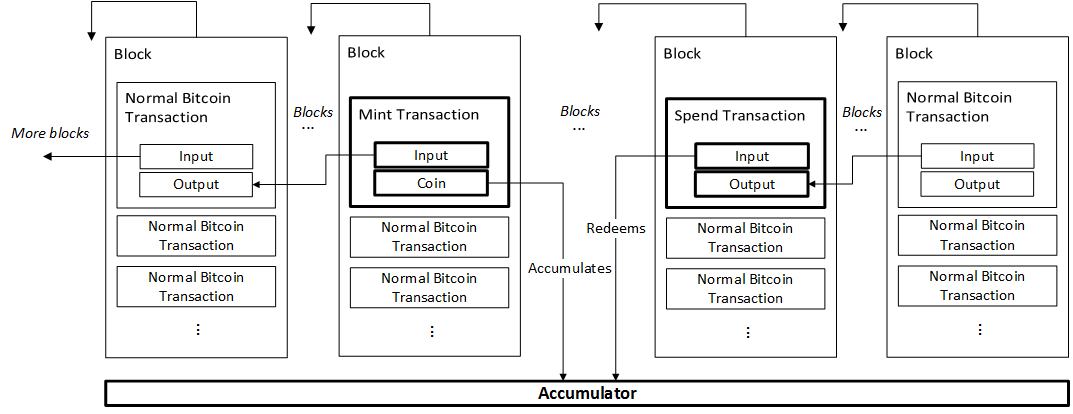
\includegraphics[scale=0.525]{zerocoin-transactions} 
		\caption{Links between Bitcoin \kwTransaction{}{s}, \kwTransaction{Mint }{s} and \kwTransaction{Spend }{s}}
		\label{fig:zerocoin_transactions} 
	\end{center}
\end{figure}

Zerocoin is in fact a mixing protocol, where minted \kwCoin{s} act as the intermediary. When a new \kwTransaction{Mint }{s} is published on the Blockchain, the minted \kwCoin{} $c$ is mixed with the rest of the previously minted \kwCoin{s} in the Accumulator. When a \kwTransaction{Spend }{} is published on the on the Blockchain, the only information available to the public is that one of all the previously minted \kwCoin{s} has been redeemed to a public key address as the redeemed \kwCoin{} is not revealed. Even though the serial number $S$ of the redeemed \kwCoin{} is revealed to verify that it has not been spent, the secret trapdoor $r$ is private to the \kwCoin{}’s owner at all times. An adversary who only know $S$ cannot determine which $c$ is being redeemed and thus cannot link the redeemer of the Zerocoin (payee) to the user who minted this \kwCoin{} (payer). Hence the anonymity set in Zerocoin is all of the minted and unredeemed \kwCoin{s} in history, which is much larger than the anonymity sets in the traditional Bitcoin mixing protocols (\S\ref{sec:2-Dedicated Mixing Services and Decentralised Mixing}). Therefore Zerocoin achieves a much higher level of anonymity compared to these protocols.

\subsubsection{Drawbacks}
\label{sec:2-Zerocoin Drawbacks}
However Zerocoin is not a perfect system. Some of the drawbacks of Zerocoin are listed below:

\begin{enumerate}
	\item \kwCoin{s} can only have fixed denominations, making payments less flexible. The reason behind the fixed denominations is to ensure that adversaries find it hard to match transaction amounts between Mint and \kwTransaction{Spend }{s} to determine links between them. This is largely similar to why transaction amounts in traditional mixing protocol must be uniform for all participants (\S\ref{sec:2-Dedicated Mixing Services and Decentralised Mixing}). 
	\item There is no provision to transfer a \kwCoin{} to a payee directly, and actual payments still need to be done in Bitcoins. Every time a payer wants to make a payment, he needs to redeem a \kwCoin{} to Bitcoins via a \kwTransaction{Spend }{}, and make the payment using the Bitcoins via a normal Bitcoin \kwTransaction{}{}. If the payee wants to make an anonymous payment again using the received Bitcoins, he must first mint some \kwCoin{s} via a \kwTransaction{Mint }{} and then redeem them via a \kwTransaction{Spend }{}. Thus \kwCoin{s} need to be constantly minted and redeemed to cater for multiple anonymous transactions. This makes anonymising transactions using Zerocoin cumbersome. 
	\item The payment amounts, payment addresses and the timings of Zerocoin transactions are still publicly available on the Blockchain. This means that Zerocoin is still exposed to side channel attacks (\S\ref{sec:1-Side Channels Attacks}).
	\item Zerocoin \kwTransaction{Spend }{s} are much larger in size (50KB) compared to Bitcoin \kwTransaction{}{s} (1KB) due to the large size of the NIZK proofs that are used to prove the ownership of \kwCoin{s}. This is undesirable in a peer-to-peer digital currency network. Firstly, since all nodes in the network maintains a copy of the Blockchain, large transactions sizes increase the storage requirement of nodes. Secondly, large transactions also take longer time to be propagated in the peer-to-peer network, which slows down the confirmation of transactions and the overall performance of the system.
\end{enumerate}

\subsection{Zerocash}
\subsubsection{Protocol}
\label{sec:2-Zerocash Protocol}
Zerocash is purported to be an improvement of Zerocoin. It is built on the same principles as Zerocoin, where a \kwTransaction{Mint }{} create some \kwCoin{s} and a Pour transaction (Similar to \kwTransaction{Spend }{} in Zerocoin) spends a minted \kwCoin{} without disclosing which \kwCoin{} is spent. Instead of using the NIZK proofs in Zerocoin to prove ownership of \kwCoin{s}, Zerocash does this by using zero-knowledge Succinct Non-interactive Arguments of Knowledge (zk-SNARKs) \cite{Ben-sasson2013}. As zk-SNARKs is extremely complex and a relatively new field, this research is not able to describe how the proof works. However its features is sufficient to evaluate Zerocash as a protocol. The improvements in Zerocash from Zerocoin that are made possible by zk-SNARKs are listed below:

\begin{enumerate}
	\item The size of the proofs for the ownership of \kwCoin{s} in Zerocash is reduced from 45KB to 288B. As such Zerocash transactions have similar size as the standard Bitcoin \kwTransaction{}{s} (1KB). 
	\item The time taken to verify a \kwTransaction{Pour }{} in Zerocash is reduce by 98.6%.
	\item Zerocash transactions hide all transaction details. The only information that is publicly available in a transactions are the zk-SNARKs proofs to verify the transactions. Hence one can only observe the existence of a transaction on the Blockchain and other information such as transaction amounts and payment addresses are hidden. This makes side channel attacks (\S\ref{sec:1-Side Channels Attacks}) impossible.
	\item Zerocash supports arbitrary denominations since the transaction amounts are hidden and cannot be exploited by side channel attacks.
	\item Zerocash allows minted \kwCoin{s} to be directly transferred from payer to payee. There is no need to redeem a \kwCoin{} into Bitcoins before payments can be made like in Zerocoin.
\end{enumerate}

\subsubsection{Drawbacks}
\label{sec:2-Zerocash Drawbacks}

Though seemingly superior, Zerocash also has the following weaknesses when compared to Zerocoin:

\begin{enumerate}
	\item The theoretical foundation of Zerocash has not be proven to be sound. zk-SNARKs is a relatively new area of research and its theories have not been used in practice as of 2015 \cite{narayanan2016bitcoin}. In contrast, the NIZK proofs used by Zerocoin, which are based on RSA cryptography (\S\ref{sec:3-Non-Interactive Zero Knowledge (NIZK) Proofs}), has been widely tested and proven for many years. 
	\item Zerocash requires a huge set of parameters (over 1GB) for the zk-SNARKs proofs. This places a huge storage constraint for anyone who wishes to use Zerocash, and makes deployment of Zerocash on mobile devices challenging. In contrast, Zerocoin only requires a single parameter of about 2.5KB for its NIZK proofs.
	\item The construction of the zk-SNARKs proofs in Zerocash computationally expensive. Specifically, it takes 2 minutes to construct the proofs in a \kwTransaction{Pour }{} using an Intel Core i7 3.40GHz processor with 16GB of RAM. This means that a user of Zerocash needs to wait for 2 minutes before he/she can create a transaction on a high-end PC. This makes Zerocash impractical for mobile devices with lower processing power. In contrast, on a machine that has similar processing power as the above mentioned Intel Core i7 processor, Zerocoin only requires 0.7s to construct a \kwTransaction{Spend }{}.
\end{enumerate}

\subsection{Selection Zerocoin as the Subject of Research}
\label{sec:2-Selection Zerocoin as the Subject of Research}
A summary of the key features of Zerocoin and Zerocash is listed in Table~\ref{tab:zerocash_zerocoin_keyfeatures}.

\begin{table}[H]
	\centering \small
	\begin{tabular}{ p{5.5cm} | p{4.25cm} | p{4.25cm} }
		
		& \textbf{Zerocoin} & \textbf{Zerocash} \\ 		
		\hline
		\hline
		\textbf{Technology} & 
		RSA cryptography. Mature and proven in practice. & 
		zk-SNARKs. New and not implemented in practice. \\	
		\hline
		\textbf{Level of anonymity} & Payment amount, timing and addresses are public. Susceptible to side channel attack. & Only transaction timing is public, hides all other transaction information. Side channel attack is not possible. \\
		\hline
		\textbf{Denomination} & Fixed & Arbitrary \\ 
		\hline
		\textbf{Direct payment using \kwCoin{s}} & No & Yes \\
		\hline
		\textbf{Size of parameters} & 2.5KB & 1GB \\	
		\hline
		\textbf{Size of proof} & 45KB & 288B \\
		\hline
		\textbf{Time taken to construct the proofs in a \textit{Spend/Pour transaction }on a high end processor} & 2 minutes & 0.7s \\
		\hline
		\textbf{Time taken to verify the proofs in a \textit{Spend/Pour transaction} on a high end processor} & 300ms & 5.7ms \\
		
	\end{tabular}
	\caption{Key features of Zerocoin and Zerocash}
	\label{tab:zerocash_zerocoin_keyfeatures}
\end{table}


Zerocash definitely has much more to offer in terms of privacy and features. However Zerocash requires large storage and a long time to construct transactions even on high-end processors, and thus may face challenges running on clients that increasingly consist of mobile devices. Though the transaction sizes of Zerocoin are relatively large and may impose higher load on the peer-to-peer network, the overall storage and processing requirements of Zerocoin for both the clients and the network is still moderate. Slight improvements in Zerocoin’s performance can make it a very practical protocol. 

In addition, the technology behind Zerocash is also not mature. Literature on zk-SNARKs is both sparse and complex, while literature on NIZK proofs are readily available and well documented \cite{Zcoin2016}. This makes research on Zerocoin more productive compared to Zerocash. Moreover the theoretical basis for Zerocash is uncertain due to the lack of implementation of zk-SNARKs in real-life applications, while Zerocoin is theoretically reliable as it uses NIZK proofs which are tested and proven. 

Most importantly, the full anonymity provided by Zerocash may be undesirable. This is because full anonymity removes a key feature of the Blockchain, which is that the peer-to-peer network can collectively audit the public transactions. If payment amounts in transactions are hidden, any bugs or attacks that cause \kwCoin{s} to be wrongly created will go unnoticed on the Blockchain. This can cause hyperinflation of Zerocash and render the system obsolete \cite{Zcoin2016}. Thus as promising as it seems, Zerocash has its caveats and its implications as a real-life digital currency system are unknown. 

Taking into account the above considerations, Zerocoin is a more attractive area of research due to its performance, the accessibility of literature and its potential application. Hence the rest of this research devotes to analysing Zerocoin in detail and finding ways to improve its performance, so that it can be a practical anonymous digital currency system. 

\ifpdf
\graphicspath{{Chapter3/Figs/}}
\else
\graphicspath{{Chapter3/Figs/}}
\fi

\chapter{Analysis of Zerocoin}
\label{ch:Analysis of Zerocoin}
This chapter delves into the data structures and algorithms of Zerocoin and analyses the reasons behind some of its key weaknesses. A basic understanding of Zerocoin and the issues of privacy detailed in Chapter \ref{ch:Privacy in Bitcoin} and \ref{ch:Methods to Improve Privacy in Digital Currencies} are needed to appreciate the rest of this chapter. Unless otherwise stated, all technical information on Zerocoin is obtained from the original Zerocoin paper \cite{Miers2013}.

\section{Construction of Zerocoin}
\subsection{Coin as a Pederson Commitment}
\label{sec:3-Coin as a Pederson Commitment}
The key element in Zerocoin is the \kwCoin{} that is minted and redeemed in Mint and \kwTransaction{Spend }{s}. A \kwCoin{} $c$ is a Pedersen commitment \cite{Pedersen1992} of a serial number $S\in\expIntGroup{\varQComm}$ and a random trapdoor $r\in\expIntGroup{\varQComm}$ in the form $c=\expPedCommCoin\bmod{\varPComm}$. $\varPComm$ and $\varQComm$ are large primes and $\varGComm$ and $\varHComm$ are generators of the sub-group of $\expIntGroup{\varQComm}$ multiplicative group $\expMulGroup{\varPComm}$. That is to say $\varGComm^0,\varGComm^1,...,\varGComm^{\varQComm}\bmod{\varPComm}$ and $\varHComm^0,\varHComm^1,...,\varHComm^{\varQComm}\bmod{\varPComm}$ produce two sequences of distinct numbers. To satisfy this property, $\varGComm^{\varQComm} \bmod{\varPComm}=1$ and $\varHComm^{\varQComm} \bmod{\varPComm}=1$ and thus $\varQComm$ divides $\varPComm-1$ by Fermat’s Little Theorem. In Zerocoin, $\varPComm$ and $\varQComm$ are prime numbers of 1024 and 256 bits respectively \footnote{Based on the security recommendations in Section VI(B) of the Zerocoin paper \cite{Miers2013}.}, and $\varGComm$ and $\varHComm$ are computed based using the algorithm defined in the Federal Information Processing Standards (FIPS) 186-34 \cite{InformationTechnologyLaboratory2009}. For simplicity of presentation, the Pedersen commitment will be written as $c=\expPedCommCoin$, where modulus $\varPComm$ is implied for generators $\varGComm$ and $\varHComm$. 

In Zerocoin, a single set of $\varGComm,\varHComm,\varPComm,\varQComm$ is generated once as public parameters during set up, and is subsequently used by all users. To mint a \kwCoin{}, a user generates a random serial number $S\in\expIntGroup{\varQComm}$ and another random trapdoor $r\in\expIntGroup{\varQComm}$, computes a Pedersen commitment $c=\expPedCommCoin$ and include $c$ in the \kwTransaction{Mint }{}. $S$ is kept secret when the \kwTransaction{Mint }{} is created and is subsequently revealed in the \kwTransaction{Spend }{} to prove the ownership of $c$ (\S\ref{sec:3-Serial Number Signature of Knowledge}), while $r$ is always secret to the creator of the \kwTransaction{Mint }{}. 

After the \kwTransaction{Mint }{} is verified and published on the Blockchain, everyone can see that the creator of the transaction has minted $c$. Theoretically, an adversary can “steal” a \kwCoin{} by obtaining $S$ and $r$ from the public $c$ and creating a valid \kwTransaction{Spend }{} using $S$ and $r$. However the adversary can only succeed with negligible probability in practice as solving $S$ and $r$ from a known $c$ where $c=\expPedCommCoin$ is believed to be hard under the Discrete Logarithm assumption \cite{Paar2010}. Due to this property, it is also hard to solve $c$ from $S$ without the knowledge of $r$. Since $r$ is secret to the owner of the \kwCoin{} at all times, an adversary is also unable to attribute the $S$ in the \kwTransaction{Spend }{s} to a $c$ in the \kwTransaction{Mint }{s} on the Blockchain. This preserves the anonymity property that the redeemer (payee) of a \kwCoin{} cannot be linked to its creator (payer).

\subsection{Public Accumulator}
\label{sec:3-Public Accumulator}
An accumulator “summarises” a large number of values into one value, and given a short witness a specific value can be proven to be accumulated in the accumulator. The accumulator in Zerocoin is a public data structure that contains every minted \kwCoin{} in history. As such, given a witness any nodes in the peer-to-peer network can verify that a \kwCoin{} has been minted using the accumulator. The size of the accumulator remains constant as more \kwCoin{s} are accumulated, thus it can be distributed and stored efficiently by the peer-to-peer network. The accumulator used in Zerocoin is a dynamic accumulator proposed by Camenisch and Lysyanskaya \cite{JanCamenisch12002} that extends the study by Baric and Pfitzmann \cite{BariC1997}. The 3 main functions provided by this accumulator scheme are explained below. 

$\eqnAccum{u}{C}$ accumulates a set of \kwCoin{s} $C=\lbrace \expOneToN{c}{n} \mid c_i \in [A,B] \wedge c_i \: is \: prime \rbrace$ using parameters $(N,u)$ to produce an accumulator $A=u^{\expOneToN{c}{n}}\bmod{N}$. Like the parameters used in the Pedersen commitment for \kwCoin{s} (\S\ref{sec:3-Coin as a Pederson Commitment}), $(N,u)$ are public parameters that are generated once during set up. $N$ is a product of 2 large primes while $u$ is a quadratic residue modulo $N$ \footnote{A quadratic residue modulo N is the square of any integer modulo N.}. $N$ is recommended is to be 3072 bits long \footnote{Based on the security recommendations in Section VI(B) of the Zerocoin paper \cite{Miers2013}.}. $\mathfrak{A}$ and $\mathfrak{B}$ \footnote{$\expAFrak,\expBFrak$. $k'$ and $k''$ are set at 160 and 128 respectively. The reasons behind these values can be found in \cite{Miers2013} and \cite{JanCamenisch12002}.} defines the range of the values that an accumulated \kwCoin{} $c$ can take. In addition, $c$ must be prime before it can be accumulated. Hence when minting a new \kwCoin{}, different $S$ and $r$ must be tried until $c=\expPedCommCoin$ satisfies the above constraints. 

Every time a new \kwCoin{} is successfully minted, nodes will accumulate the new \kwCoin{} into the public accumulator. Due to the construction of the dynamic accumulator, a new \kwCoin{} $c_{new}$ can be incrementally accumulated \cite{JanCamenisch12002} into the previous accumulator $A$ using $\eqnAccum{A}{\{c_{new}\}}$. Thus when updating the accumulator, one do not need to recompute $u^{\expOneToN{c}{n}c_{new}}\bmod{N}$ but simply compute $A^{c_{new}}\bmod{N}$ using the latest $A$, making accumulation efficient. Zerocoin proposes that each \kwBlock{} contains an accumulator called the accumulator checkpoint that contains all the \kwCoin{s} minted up till that \kwBlock{}. This way nodes do not need to compute the accumulator from scratch, and can choose an accumulator checkpoint from any \kwBlock{} and incrementally accumulate the \kwCoin{s} minted after that \kwBlock{} to obtain the latest accumulator value.

For a \kwCoin{} $c\in C$, $\eqnGenWit{c}{w}$ produces a witness $w=\eqnAccum{u}{C\setminus\{c\}}$. That is, $is$ an accumulation of all the \kwCoin{s} in $C$ except $c$. In Zerocoin, $C$ is the set of all minted \kwCoin{s} in history. With $w$, one can verify that that $c$ is in $C$ using $\eqnAccVer{c}$, where $A=\eqnAccum{u}{C}$. $AccVerify$ returns 1 if and only if $A=w^{c}\bmod{N}$ and $c$ is a valid \kwCoin{} ($c$ is prime and $c\in[\mathfrak{A},\mathfrak{B}]$). It can be seen that $A=w^{c}\bmod{N}$ is the correct verification equation as $A=\eqnAccum{u}{C}=u^{\expOneToN{c}{n}c}\bmod{N}=(u^{\expOneToN{c}{n}})^c\bmod{N}=w^{c}\bmod{N}$. To ensure security, $A$ should be independently computed by each verifier, which can be achieved efficiently using the incremental method described in the previous paragraph.

In Zerocoin, $GenWitness$ is used by the creator of a \kwTransaction{Spend }{} to create a witness to prove that the redeemed \kwCoin{} is in the accumulator. $AccVerify$ is used by nodes in the Zerocoin network to verify that claim when validating the \kwTransaction{Spend }{}. However $AccVerify$ is used only in principle and not directly, because $w$ and $c$ are not revealed to the verifier in a \kwTransaction{Spend }{} in order to keep $c$ unkown. Why and how the \kwTransaction{Spend }{} is verified without the knowledge of $w$ and $c$ is discussed in \S\ref{sec:3-Accumulator Proof of Knowledge}.

\subsection{Non-Interactive Zero Knowledge (NIZK) Proofs}
\label{sec:3-Non-Interactive Zero Knowledge (NIZK) Proofs}
\subsubsection{Interactive Zero Knowledge Proofs}
\label{sec:3-Interactive Zero Knowledge Proofs}
Zerocoin relies heavily on NIZK proofs, which are a subset of zero-knowledge (ZK) proofs. ZK proof is a proof of the knowledge of an element without disclosing any information beyond the legitimacy of the proof \cite{Kiayias} The formal notation of ZK proof introduced by Camenisch and Stadler \cite{Camenisch1997a} is as follow:

$$ZKPoK\{(w):statement\ proving\ knowledge\ of\ w\}$$

$ZKPoK$ refers to Zero-Knowledge Proof of Knowledge. The proof statement is enclosed in the curly brackets. The element in parenthesis is the information that the prover wishes to show knowledge of, but cannot be disclosed. This notation will be used for all zero knowledge proofs in this paper. 

ZK proofs often surrounds an NP-hard problem. In general, a prover wants to prove that he has a secret solution $w$ to the NP-hard problem $y$. The prover first sends a random problem $t$ that has a solution $v$ that is unrelated to $w$. The verifier then sends a random challenge $\varChallenge$ to the prover, and the prover replies with a response $s$ that looks random but in fact is a combination of $v$, $w$ and $\varChallenge$. The verifier verifies the proof by composing $s$ with $\varChallenge$ and the original problem $y$. $s$ is constructed in a way such that if the prover knows $w$, it will cancel out $y$, leaving behind only the random problem $t$. Hence by checking that the result of the proof is $t$ the verifier is able to verify the proof, but does not learn anything about $w$ since all he sees are random values. The above is a form of interactive ZK proof which involves the verifier communicating the challenge $\varChallenge$ to the prover. A simple example of an interactive ZK proof for the knowledge of discrete logarithm can be found online \cite{Unknown2016}. This proof is chosen as an example as it is closely related to the proofs used in the Zerocoin protocol.

\subsubsection{Transforming Interactive Zero Knowledge Proofs to NIZK Proofs}
\label{sec:3-Transforming Interactive Zero Knowledge Proofs to NIZK Proofs}
NIZK proof is a special kind of ZK proof that removes the need for the verifier to interact with the prover. The prover can achieve this by a generating a challenge $\varChallenge$ from $y$ and $t$ using a random oracle \footnote{A theoretical black box that responds to every unique query with a truly random response chosen uniformly from its output domain. If a query is repeated it responds the same way every time that query is submitted. \cite{Unknown2016a}}, and treat this $\varChallenge$ as the challenge that the verifier sends in the interactive version the ZK proof. The prover then computes $s$ based on the generated $\varChallenge$ and sends the proof containing $y$, $t$ and $s$ to the verifier. Upon receiving the proof, the verifier recomputes $\varChallenge$ from the received $y$ and $t$ using the random oracle, and verifies the proof in the same way as the interactive version of the ZK proof. Since there is no interaction between the prover and the verifier, the NIZK is achieved. 

The Fiat-Shamir heuristics \cite{Fiat1987} is a popular technique to transform interactive ZK proofs into NIZK proofs. Using the Fiat-Shamir heuristics, the random oracle is implemented as a cryptographic hash function \cite{Bellare1993}, and $\varChallenge$ is obtained by hashing $y$ and $t$ together with and other parameters. The NIZK proofs used in Zerocoin and the proofs proposed by this research all use the Fiat-Shamir heuristics in one way or another. The same online resource that illustrates interactive ZK proof for the knowledge of discrete logarithm also shows how the proof can be modified into a NIZK form using the Fiat-Shamir heuristics \cite{Unknown2016}. 

\subsubsection{Properties of Zero-Knowledge Proofs}
\label{sec:3-Properties of Zero-Knowledge Proofs}
All ZK proofs (NIZK proofs included) need to fulfil the below properties \cite{Kiayias}:
\begin{enumerate}
	\item \textbf{\textit{Completeness}}: If the prover indeed knows the secret $w$, and both the prover and verifier follow the procedures of the proof, then the proof will always be verified.
	\item \textbf{\textit{Soundness}}: If the prover does not know the secret $w$, and both the prover and verifier follow the procedures of the proof, then the proof will not be verified. This property can be proven if a hypothetical program called the knowledge extractor that can extract $w$ from the prover using two accepting proofs that uses the same $t$ but different $\varChallenge$ and $s$. In order to do this, the knowledge extractor has access to the prover’s program (but not the $w$ itself) and can “rewind” the proof to obtain another set of $\varChallenge$ and $s$. The success of the knowledge extractor is needed to prove for soundness because if a prover who does not know $w$ manages to prove the knowledge of $w$, there is no way that a knowledge extractor can extract a $w$ that is non-existent in the proof.
	\item \textbf{\textit{Statistical Zero-Knowledge}}: The verifier does not gain any knowledge after interacting with the prover. This can be proven if a hypothetical program called a simulator with no knowledge of the secret $w$, is able to generate a response $s'$ to the challenge $\varChallenge$, such that $s'$ is statistically indistinguishable from the actual response $s$ generated by the prover. In this way the verifier does not learn anything more from the $s$ sent by the prover than from the $s$ sent by the simulator.
\end{enumerate}

\subsubsection{NIZK Proofs in Zerocoin}
\label{sec:3-NIZK Proofs in Zerocoin}
NIZK proofs are used in Zerocoin to prove the ownership of a valid unredeemed \kwCoin{} in a \kwTransaction{Spend }{}. The proof needs to be zero-knowledge so that the verifier or anyone who sees the \kwTransaction{Spend }{} does not know which \kwCoin{} is being spent. The proof also needs to be non-interactive because a \kwTransaction{Spend }{} can be verified by any node in the Zerocoin network at any time, and it is not possible for a verifier to interact with the creator of the transaction. The three NIZK proofs in a \kwTransaction{Spend }{} are:

\begin{enumerate}
	\item \textbf{\textit{Accumulator Proof of Knowledge (AccPoK)}}: Proves that a \kwCoin{} $c$ has been minted, without disclosing $c$. This is achieved by proving that $c$ is contained in the public accumulator in which every \kwCoin{} that has been minted should have been included in. Details of this proof is discussed in \S\ref{sec:3-Accumulator Proof of Knowledge}.
	\item \textbf{\textit{Serial Number Signature Proof of Knowledge (SNSoK)}}: Proves the knowledge of the serial number $S$ and the secret trapdoor $r$ that are committed in the redeemed \kwCoin{} $c$, without disclosing $r$ and $c$. Since only the owner of a \kwCoin{} knows its $S$ and $r$, this proof shows that the prover owns the \kwCoin{} being proven for. This proof also acts as a digital signature for the \kwTransaction{Spend }{}. A digital signature is needed to prevent the contents of the \kwTransaction{Spend }{}, which contains the public key address that the redeemed \kwCoin{} should be paid to, from being tampered with. Details of this proof is discussed in \S\ref{sec:3-Serial Number Signature of Knowledge}. 
	\item \textbf{\textit{Commitment Proof of Knowledge (CommPoK)}}: Proves that the \kwCoin{} being proven for in the accumulator Proof of Knowledge and the \kwCoin{} being proven for in the Serial Number Signature of Knowledge are the same \kwCoin{}. This ensures the \kwCoin{} which the prover is proving to be minted is the same \kwCoin{} that he is proving ownership for. With this proof, one cannot redeem a minted \kwCoin{} that he does not own. Details of this proof is discussed in \S\ref{sec:3-Commitment Proof of Knowledge}. 
\end{enumerate}

\subsubsection{Accumulator Proof of Knowledge}
\label{sec:3-Accumulator Proof of Knowledge}
For a \kwCoin{} to be spent, it must first be proven that the \kwCoin{} has been minted. The Accumulator Proof of Knowledge (AccPoK) proves this claim using the public accumulator which contains all the minted \kwCoin{s} in history.

As seen in \S\ref{sec:3-Public Accumulator}, the claim that a \kwCoin{} $c$ is in the set of minted \kwCoin{s} can be verified by presenting $AccVerify$ with the witness $w$. However this cannot be done directly in Zerocoin as $c$ needs to be secret in order to preserve unlinkability between the minter and the redeemer of $c$. In addition, $w$ also needs to be secret as it can be used to obtain $c$. This is possible because all the minted \kwCoin{s} in history are publicly available in the \kwTransaction{Mint }{s} on the Blockchain. An adversary can run $\eqnGenWit{c'}{w'}$ repeatedly using all $c'\in C$, where $C$ is all the minted \kwCoin{s} in history, and the $c'$ that produced a $w=w'$ is the \kwCoin{} that is being proven for. Hence to hide $c$ and $w$, the AccPoK is as such:

$$\eqnAccPoK$$

The implementation of the AccPoK is adapted from an interactive version of the proof by Camenisch and Lysyanskaya \cite{JanCamenisch12002} and modified to a non-interactive form using the Fiat-Shamir heuristics. The rest of the section describes the implementation details. 

In order to hide $c$ and $w$, the prover creates the following commitments of $c$ and $w$ using random trapdoors:

\begin{enumerate}
	\item $\varAccPoKCoinComm$, a commitment of $c$ with a random trapdoor $ \varphi\in\expIntGroup{\lfloor N/4 \rfloor}$ such that $\varAccPoKCoinComm=\varAccPoKGComm^{c}\varAccPoKHComm^{\varphi}\bmod{\varAccPoKPComm}$. $\varAccPoKGComm$ and $\varAccPoKHComm$ are generators for sub-group $\expIntGroup{\varAccPoKQComm}$ of multiplicative group $\expIntGroup{\varAccPoKPComm}^{*}$, where $\varAccPoKQComm >2\mathfrak{B}$.
	\item $\varAccPoKProofComm{c}$, another commitment of $c$ with a random trapdoor $ \eta\in\expIntGroup{\lfloor N/4 \rfloor}$ such that $\varAccPoKProofComm{c}=\varAccPoKGProof^{c}\varAccPoKHProof^{\eta}\bmod{N}$. $\varAccPoKGProof$ and $\varAccPoKHProof$ are quadratic residues modulo $N$.
	\item $\varAccPoKProofComm{w}$, a commitment of the witness $w$ with a random trapdoor $ \epsilon\in\expIntGroup{\lfloor N/4 \rfloor}$ such that $\varAccPoKProofComm{w}=w\varAccPoKHProof^{\epsilon}\bmod{N}$.
	\item $\varAccPoKProofComm{r}$, a commitment of $\epsilon$ with a random trapdoor $\zeta\in\expIntGroup{\lfloor N/4 \rfloor}$ such that $\varAccPoKProofComm{r}=\varAccPoKGProof^{\epsilon}\varAccPoKHProof^{\zeta}\bmod{N}$.
\end{enumerate}

Like the parameters used in the accumulator (\S\ref{sec:3-Public Accumulator}), $\varAccPoKGComm,\varAccPoKHComm,\varAccPoKGProof,\varAccPoKHProof,\varAccPoKPComm,\varAccPoKQComm$ are public parameters that are generated once during set up. For simplicity of presentation, the modulus of the above commitments are omitted and implied. With these commitments, the prover implements the AccPoK by constructing a NIZK proof that shows that $\varAccPoKCoinComm$ and the accumulator $A$ contains the same $c$ in the following form:

\eqnAccPoKActual

The proof follows the standard flow of a NIZK proof described in \S\ref{sec:3-Transforming Interactive Zero Knowledge Proofs to NIZK Proofs}. Since there are 8 sub proofs in the NIZK proof, the prover first commits some random values $v_i$ to create commitments $\varAccPoKCoinComm,\varAccPoKProofComm{c},\varAccPoKProofComm{w},\varAccPoKProofComm{r}$ that are not related to,for each of the sub-proof. Following the principle of the Fiat-Shamir heuristics, the prover computes the challenge string $\varChallenge=H(\expConcatAccPoK)$ \footnote{$H$ denotes the SHA-256 hash function used by Zerocoin. $\|$ denotes a concatenation operation} and further computes $s_i$ that correspond to each $t_i$ using $\varChallenge$. The final $\varAccPoKCoinComm,\varAccPoKProofComm{c},\varAccPoKProofComm{w},\varAccPoKProofComm{r},t_i,s_i$ are written into the \kwTransaction{Spend }{} and broadcasted to the Zerocoin network to be verified. Upon receiving the \kwTransaction{Spend }{}, the nodes re-computes $\varChallenge=H(\expConcatAccPoK)$ using the received $\varAccPoKCoinComm,\varAccPoKProofComm{c},\varAccPoKProofComm{w},\varAccPoKProofComm{r},t_i,s_i$ and the public parameters $\varAccPoKGComm,\varAccPoKHComm,\varAccPoKGProof,\varAccPoKHProof$,. The verifier then verifies the proof by checking if each received $t_i$ equals to the $t'_i$ computed from $\varChallenge$ and $s_i$ using some verification formulas. The verification formulas are detailed in Appendix A of \cite{JanCamenisch12002}. The completeness, soundness and statistical zero-knowledge properties of the proof are also detailed in the \S3.3 of the same study.

\subsubsection{Serial Number Signature of Knowledge}
\label{sec:3-Serial Number Signature of Knowledge}
Proving that a \kwCoin{} has been accumulated in the public accumulator only shows that the prover knows some \kwCoin{} has been minted, but does not legitimise his ownership of the \kwCoin{}. Anyone who looks at the Blockchain can simply take a \kwCoin{} from any past \kwTransaction{Mint }{s}, obtain a witness for the \kwCoin{} using $GenWitness$ and construct a valid AccPoK for that \kwCoin{}. Hence, the creator of a \kwTransaction{Spend }{} must also prove that he owns the redeemed \kwCoin{}. This is done using the Serial Number Signature of Knowledge (SNSoK) where the prover proves that he knows the serial number $S$ and the random trapdoor $r$ that are committed a \kwCoin{} $c$ without disclosing $r$ and $c$. Since $r$ is secret to the owner of $c$ at all times, only the owner of the $c$ can produce a valid proof. This proof is a “signature” because it binds to the other contents of the \kwTransaction{Spend }{} such as the public key address of the payee. As the SNSoK becomes invalid once the contents of the \kwTransaction{Spend }{} changes, adversaries cannot tamper with the \kwTransaction{Spend }{}. Given the above objectives and constraints, the SNSoK in Zerocoin is as such:

$$\eqnSNSoK$$

The $m$ enclosed in the square brackets denotes the contents in the \kwTransaction{Spend }{} to be signed. As the serial number $S$ of the redeemed $c$ is disclosed in the proof, the trapdoor $r$ must be kept secret to prevent $c$ from being computed by observers of the Blockchain. The implementation of the SNSoK is adapted from the proof by Camenisch \cite{No1998}.

In order to hide $c$, the prover creates $y$, a Pedersen commitment of $c$ using a random trapdoor $z\in\expIntGroup{\varQSok}$, such that $y=\expSoKCoinComm{c}\bmod{\varPSok}=\expSoKCoinComm{\expPedCommCoin}\bmod{\varPSok}$. As per Pedersen commitment scheme, $\varGSok$ and $\varHSok$ are generators of the sub-group $\expIntGroup{\varQSok}$ of multiplicative group $\expMulGroup{\varPSok}$, and $\varQSok|\varPSok-1$. As the exponent in a Pederson commitment must be an element of $\expIntGroup{q}$ \cite{Pedersen1992}, $c\in\expIntGroup{\varQSok}$ and since $c$ is a value modulo $\varPComm$ (\S\ref{sec:3-Coin as a Pederson Commitment}), it is required that $\varQSok=\varPComm$. Like the parameters used in the Pedersen commitment for \kwCoin{s} (\S\ref{sec:3-Coin as a Pederson Commitment}), $\varGSok,\varHSok,\varPSok,\varQSok$ are public parameters that are generated once during set up. For simplicity of presentation, the modulus $\varPSok$ is omitted and implied for $\varGSok$ and $\varHSok$. With $y$, the prover implements the SNSoK by constructing a NIZK proof that shows that $y$ contains a $c$ that is a commitment to the serial number $S$ and trapdoor $r$ in the following form:

$$\eqnSNSoKActual$$

The flow of the NIZK proof is largely similar to the standard NIZK proof under the Fiat-Shamir heuristics described in \S\ref{sec:3-Non-Interactive Zero Knowledge (NIZK) Proofs}, but has a slightly different way of computing and using the challenge $\varChallenge$. The prover first creates $t_i$ for $i$ from 0 to $\varLambdaSec$ using random numbers $u_i\in\expIntGroup{\varQComm}$ and $v_i\in\expIntGroup{\varQSok}$ such that $t_i=\varGSok^{\varGComm^{S}\varHComm^{u_i}}\varHSok^{v_i}$. To ensure security, the Zerocoin paper recommends that $\varLambdaSec=80$ \footnote{Based on the security recommendations in Section VI(B) of the Zerocoin paper \cite{Miers2013}.}. Following the principle of the Fiat-Shamir heuristics, the prover then computes the challenge string $\varChallenge=H(\expConcatSNSoK)$. The inclusion of $m$ in the hash $\varChallenge$ ensures that the contents of the \kwTransaction{Spend }{} is bound to the challenge string. Any tampering with $m$ will cause $\varChallenge$ to be invalid and the proof fail. Thus $\varChallenge$ also serves as the signature for $m$. Using $\varChallenge$ the prover then computes $s_i$ and $s'_i$ in the following manner:

\begin{algorithm}
	\begin{algorithmic}[H]
		\For{$i\gets 1, \varLambdaSec$}
		\If{$i^{th}$ bit in $\varChallenge=0$}
		\State $s_i=(u_i-r)$; $s'_i=(v_i-z\varHComm^{u_i-r})$ 
		\Else
		\State $s_i=u_i$; $s'_i=v_i$
		\EndIf
		\EndFor
	\end{algorithmic}
\end{algorithm}	

The prover writes $y,\varChallenge,t_1,\cdots,t_{\varLambdaSec},s_1,\cdots,s_{\varLambdaSec},s'_1,\cdots,s'_{\varLambdaSec}$ and the transaction content $m$ into the \kwTransaction{Spend }{} and broadcast it to the Zerocoin network to be verified. Upon receiving the \kwTransaction{Spend }{}, the nodes computes $\varChallenge'=H(\expConcatPrimeSNSoK)$ where:

\begin{algorithm}
	\begin{algorithmic}[H]
		\For{$i\gets 1, \varLambdaSec$}
		\If{$i^{th}$ bit in $\varChallenge'=0$}
		\State $t'_i=y^{\varHComm^{s_i}}\varHSok^{s'_i}$ 
		\Else
		\State $t_i=\varGSok^{\varGComm^{S}\varHComm^{s_i}}\varHSok^{s'_i}$
		\EndIf
		\EndFor
	\end{algorithmic}
\end{algorithm}	

The proof is verified if and only if $\varChallenge'$ equals to the $\varChallenge$ received. In order for $\varChallenge'=\varChallenge$, it must be the case that $t_i=t'_i$ for $i$ from 1 to $\varLambdaSec$. In addition, the $m$ used to compute $\varChallenge'$ must also be the original $m$ used to compute $\varChallenge$, and thus $\varChallenge$ acts as the signature that preserves the integrity of $m$. The details of the SNSoK are taken from Appendix B of the Zerocoin paper. The completeness, soundness and statistical zero-knowledge properties of the proof are also detailed in the same paper.

\subsubsection{Commitment Proof of Knowledge}
\label{sec:3-Commitment Proof of Knowledge}
The AccPoK and SNSoK independently proves a certain property of a \kwCoin{}. However with only these two proofs, nothing is stopping one from constructing an AccPoK and a SNSoK for two different \kwCoin{s}. A dishonest user can exploit this by constructing a valid SNSoK for an arbitrary \kwCoin{} using an arbitrary serial number and secret trapdoor, and a valid AccPoK for any minted \kwCoin{} on the Blockchain (\S\ref{sec:3-Accumulator Proof of Knowledge}). Since the \kwCoin{s} in the two proofs are not known to the verifying nodes, the dishonest user is able to spend the arbitrary \kwCoin{}, and claim that it is the minted \kwCoin{} without being found out. This is analogous to the ability to printing money in real life. Hence there must be some way to ensure that the \kwCoin{s} being proven for in the AccPoK and SNSoK are the same \kwCoin{}. This is achieved using the Commitment Proof of Knowledge (CommPoK), where the prover proves that that commitment of the \kwCoin{} $\varAccPoKCoinComm=\varAccPoKGComm^{c}\varAccPoKHComm^{\varphi}$ used in the AccPoK contains the same $c$ as the commitment of the \kwCoin{} $y=\expSoKCoinComm{c}$ used in the SNSoK. Hence the CommPoK is implemented in the following form:

$$\eqnCommPoK$$

The CommPoK is an extension of the proof by Camenisch to prove for the equality of two secret keys \cite{No1998}. The proof follows the standard flow of a NIZK proof described in \S\ref{sec:3-Transforming Interactive Zero Knowledge Proofs to NIZK Proofs}. The prover first creates commitments $t_1=\varAccPoKGComm^{v_1}\varAccPoKHComm^{v_2}$ and $t_2=\varGSok^{v_1}\varHSok^{v_3}$ using random numbers $v_1,v_2,v_3$. Following the principle of the Fiat-Shamir heuristics, the prover computes the challenge string $\varChallenge=H(\expConcatCommPoK)$ and further computes $s_1=v_1+c\varChallenge$, $s_2=v_2+\varphi\varChallenge$ and $s_3=v_3+z\varChallenge$. The prover then includes $\varAccPoKCoinComm,y,t_1,t_2,s_1,s_2,s_3$ in the \kwTransaction{Spend }{} together with the other proofs and broadcasts the transaction to the Zerocoin network. Upon receiving the proof in the \kwTransaction{Spend }{}, the verifying nodes re-compute $\varChallenge=H(\expConcatCommPoK)$ using the received $\varAccPoKCoinComm,y,t_1,t_2$ and the public parameters $\varAccPoKGComm,\varAccPoKHComm,\varGSok,\varHSok$. The verifier then verifies the proof by checking if both equalities $t_1=\varAccPoKGComm^{s_1}\varAccPoKHComm^{s_2}\varAccPoKCoinComm^{-\varChallenge}$ and $t_2=\varGSok^{s_1}\varHSok^{s3}y^{-\varChallenge}$ are true. The completeness, soundness and statistical zero-knowledge properties of the proof are detailed in the study by Camenisch \cite{No1998}.

\subsubsection{Public Parameters}
\label{sec:3-Public Parameters}
A summary of the public parameters used in the Zerocoin protocol is listed in Table~\ref{tab:pub_params}. These parameters only need to be generated once during the setup of the Zerocoin system, and are subsequently used by all nodes for creating and verifying transactions. 

\begin{table}[H]
	\centering \small
	\begin{tabular}{ l | m{2cm} | m{2.5cm} | m{5.5cm} }
		
		& \textbf{Public Parameter} & \textbf{Recommended value/size} & \textbf{Properties}\\ 		
		\hline
		\hline
		\multirow{4}{*}{\textbf{Coin commitment}} 
		& $\varPComm$ & 1024 bits & $\varQComm|\varPComm-1$ \\
		& $\varQComm$ & 256 bits & $\varQComm|\varPComm-1$ \\
		& $\varGComm$ & N.A. & Generator for sub-group $\expIntGroup{\varQComm}$ of multiplicative group $\expMulGroup{\varPComm}$ \\
		& $\varHComm$ & N.A. & Generator for sub-group $\expIntGroup{\varQComm}$ of multiplicative group $\expMulGroup{\varPComm}$ \\
		\hline
		\multirow{4}{*}{\textbf{Public Accumulator}}
		& $N$ & 3072 bits & Product of two large primes \\
		& $[\mathfrak{A},\mathfrak{B}]$ & N.A. & $[-\varPComm2^{k'+k''+2},\varPComm2^{k'+k''+2}]$ \\
		& $k$ & 160 & \\
		& $k'$ & 128 & \\
		\hline
		\multirow{6}{*}{\textbf{AccPoK/CommPoK}} 
		& $\varAccPoKPComm$ & N.A.& $\varAccPoKQComm|\varAccPoKPComm-1$ \\
		& $\varAccPoKQComm$ & $>2\mathfrak{B}$ & $\varAccPoKQComm|\varAccPoKPComm-1$ \\
		& $\varAccPoKGComm$ & N.A. & Generator for sub-group $\expIntGroup{\varAccPoKQComm}$ of multiplicative group $\expMulGroup{\varAccPoKPComm}$ \\
		& $\varAccPoKHComm$ & N.A. & Generator for sub-group $\expIntGroup{\varAccPoKQComm}$ of multiplicative group $\expMulGroup{\varAccPoKPComm}$ \\
		& $\varAccPoKGProof$ & N.A. & Quadratic residue modulo $N$ \\
		& $\varAccPoKHProof$ & N.A. & Quadratic residue modulo $N$ \\
		\hline
		\multirow{5}{*}{\textbf{SNSoK/CommPoK}}
		& $\varLambdaSec$ & 80 & \\
		& $\varPSok$ & N.A. & $\varQSok|\varPSok-1$\\
		& $\varQSok$ & N.A. & Equals $\varPComm$ \\
		& $\varGSok$ & N.A. & Generator for sub-group $\expIntGroup{\varQSok}$ of multiplicative group $\expMulGroup{\varPSok}$\\
		& $\varHSok$ & N.A. & Generator for sub-group $\expIntGroup{\varAccPoKQComm}$ of multiplicative group $\expMulGroup{\varAccPoKPComm}$\\
		\hline
	\end{tabular}
	\caption{Public parameters used in Zerocoin}
	\label{tab:pub_params}
\end{table}

\section{Zerocoin Implementation: libzerocoin}
\label{sec:3-Zerocoin Implementation: libzerocoin}
The main protocols in Zerocoin have been implemented in C++ by the Zerocoin authors and the source code is publicly available on Github under the name of libzerocoin \footnote{Code repository can be accessed at https://github.com/Zerocoin/libzerocoin}. libzerocoin is not a full-fledged digital currency system. Instead, it is a library that provides the functions of setting up Zerocoin public parameters (\S\ref{sec:3-Public Parameters}), creating (\S\ref{sec:3-Coin as a Pederson Commitment}) and accumulating \kwCoin{s} (\S\ref{sec:3-Public Accumulator}) and constructing and verifying the various zero-knowledge proofs (\S\ref{sec:3-NIZK Proofs in Zerocoin}). Since libzerocoin has implemented all of the key elements of Zerocoin, it can be used to analyse the performance of the Zerocoin in isolation. More importantly, libzerocoin provides a comprehensive set of functions to generate protocol parameters and perform cryptography-related computations such as SHA-256 and modulo arithmetic on large numbers. This allows the high level protocol of Zerocoin to be modified without the need to meddle with the details, and makes implementing improvements convenient. Hence this research builds on the code base of libzerocoin to conduct tests and make potential improvements.
 
\section{Performance of Zerocoin and Areas for Improvement}
\label{sec:3-Performance of Zerocoin and Areas for Improvement}
libzerocoin has been modified to test the computational and storage requirements of the key data structures and algorithms in Zerocoin. The tests are conducted using the public parameter values and sizes recommended by the Zerocoin paper (Table \ref{tab:pub_params}). The machine used to run the tests is a \_\_\_\_. The results of the tests are shown in Table~\ref{tab:zerocoin_comp_storage}.

\begin{table}[H]
	\centering
	\begin{tabular}{ l | c | c }
		\multirow{2}{*}{} & \multicolumn{2}{c}{\textit{Average over 50 iterations}} \\
		& \textbf{Time taken} & \textbf{Size of output} \\ 		
		\hline 
		\hline
		Generation of public parameters & 849ms & 2578 bytes \\
		\hline
		Creation of one \kwCoin{} & 324ms & 199 bytes \\
		Accumulation of one \kwCoin{} & 39ms & 391 bytes (accumulator size) \\
		\hline
		Construction of one AccPoK & 146ms & \textbf{6,974 bytes} \\
		Construction of one SNSoK & 146ms & \textbf{17,420 bytes} \\
		Construction of one CommPoK & 5ms & 714 bytes \\
		\hline
		Verification of one AccPoK & \textbf{100ms} & N.A. \\
		Verification of one SNSoK & \textbf{163ms} & N.A. \\
		Verification of one CommPoK & 4ms & N.A. \\
		\hline
	\end{tabular}
	\caption{Computational and storage requirements of Zerocoin}
	\label{tab:zerocoin_comp_storage}
\end{table}

The results highlighted in bold are identified as the performance weaknesses of Zerocoin which this research aims to address. With reference to Table \ref{tab:zerocoin_comp_storage}, the next two sections elaborate on why these weaknesses are identified. 

\subsubsection{Computational Performance}
\label{sec:3-Computational Performance}
The computations that affect the performance of Zerocoin the most are those which need to be carried out by the Zerocoin peer-to-peer network. For the generation of public parameters, the Zerocoin network does no incur any computational costs since the parameters are generated once by the trusted party that sets up the system. Thus the cost of generating public parameters is not considered a performance issue. The creation of \kwCoin{s} and the construction of the NIZK proofs are carried out by Zerocoin users whenever they want to make a transaction. Even though the time taken for these operations is in the order of hundreds of milliseconds, the computation requirement is contained within the individual users. As such \kwCoin{} creation and proofs construction do not impose on the peer-to-peer network, and its relatively high computation requirement is still acceptable.

The accumulation of \kwCoin{s} is performed by all nodes in the Zerocoin network as they need the most updated accumulator value to verify \kwTransaction{Spend }{s}. Although the 39ms taken to accumulate a \kwCoin{} is not small, nodes only need to accumulate the newly minted \kwCoin{s} to the previous accumulator each time a new \kwBlock{} is received since the accumulator can be incrementally computed (\S\ref{sec:3-Public Accumulator}). As blocks are only added to the Blockchain every 10 minutes (as per Bitcoin), nodes only need to periodically accumulate a small subset of the minted \kwCoin{s} in history. With this optimisation, the computational requirement to accumulate a \kwCoin{} is acceptable. 

On the other hand, verification of NIZK proofs is done by all nodes in the Zerocoin network whenever they receive a \kwTransaction{Spend }{}. Thus the time needed to verify \kwTransaction{Spend }{s} grows linearly with the number of \kwTransaction{Spend }{s} received. The verification time of the AccPoK (100ms) and the SNSoK (163ms), which make up the bulk of the verification time of a \kwTransaction{Spend }{}, is an area of concern. In fact, the Zerocoin paper showed that the rate at which nodes verify transactions decreases by about half when only 12.5\% of all transactions in the network are \kwTransaction{Spend }{s} and the other 12.5\% and 75\% are \kwTransaction{Mint }{s} and standard Bitcoin transactions respectively \cite{Miers2013}. In addition, a node may need to verify the same \kwTransaction{Spend }{s} twice – once before it forwards the \kwTransaction{Spend }{} to its peers, and another time when a new \kwBlock{} containing the \kwTransaction{Spend }{} is received. The longer time taken by nodes to verify \kwTransaction{Spend }{s} increases the time taken for transactions to reach mining nodes and make it to the Blockchain, and slows the Zerocoin entire network. Thus, the inefficiency in verifying the AccPoK and the SNSoK is a serious limiting factor to Zerocoin’s performance, and this research aims to reduce the time taken to verify these proofs.

\subsubsection{Storage Requirements}
\label{sec:3-Storage Requirements}
Each node in Zerocoin stores a single copy of the public parameters, thus the 2.5KB of storage required by the public parameters is negligible. The other Zerocoin data structures need to be stored by nodes on a \kwTransaction{}{} or \kwBlock{} basis as part of the Blockchain, and their sizes affect the storage requirements of Zerocoin significantly. The rest this section uses Bitcoin as a point of reference to demonstrate the storage implications of Zerocoin.

The accumulator is stored on a \kwBlock{} level. As of October 2016, the average size of one \kwBlock{} in Bitcoin is about 0.8MB \cite{Blockchain.info2016}. Thus an additional accumulator of 391 bytes for each \kwBlock{} has negligible effect on the \kwBlock{} size. On the other hand, a \kwCoin{} is stored in each \kwTransaction{Mint }{}, while the AccPoK, SNSoK and CommPoK are stored in each \kwTransaction{Spend }{}. As of 2015, the average size of one standard Bitcoin \kwTransaction{}{} in is 566 bytes \cite{TradeBlock2015}. For simplicity of analysis, the Zerocoin data structures are added to the standard Bitcoin \kwTransaction{}{} to estimate the size of Zerocoin transactions. As such, a \kwTransaction{Mint }{} is bigger than a Bitcoin \kwTransaction{}{} by the size of a \kwCoin{} (199 bytes), and a \kwTransaction{Spend }{} is bigger than a Bitcoin \kwTransaction{}{} by the total size of the AccPoK, SNSoK and CommPoK (25KB). This means that a \kwTransaction{Mint }{} increases transaction size by 35\% while a \kwTransaction{Spend }{} increases transaction size by 4,400\%. 

While a 35\% increase in size for a \kwTransaction{Mint }{} is still reasonable, a 44-fold increase in size for a \kwTransaction{Spend }{} is undesirable. To illustrate, if \kwTransaction{Spend }{s} make up just 10\% of all the transactions on the Blockchain, the total size of the transactions on the Blockchain will increase by 4.4 times. Since transactions make up the bulk of Blockchain stored in every node, the Zerocoin protocol imposes an enormous storage requirement compared to Bitcoin. In addition, the large size of the Zerocoin transaction also slows down the propagation of transactions in the network. As a result, Zerocoin transactions takes longer to reach the mining nodes and make it to the Blockchain, and slows down the entire Zerocoin network. Since the \kwTransaction{Spend }{} contributes significantly the storage requirements and the AccPoK (6974 bytes) and the SNSoK (17,420 bytes) make up the bulk of a \kwTransaction{Spend }{}, this research aims to reduce the size of the AccPoK and SNSoK to improve the overall performance of Zerocoin.


\ifpdf
\graphicspath{{Chapter4/Figs/}}
\else
\graphicspath{{Chapter4/Figs/}}
\fi

\chapter{Contribution of Research}
\section{Objectives}
\label{sec:4-Contribution of Research Objectives}
Based on the performance analysis of the Zerocoin in \S\ref{sec:3-Performance of Zerocoin and Areas for Improvement}, this research aims to improve these aspects of Zerocoin: 

\begin{enumerate}
	\item Reduce the time taken to verify the Accumulator Proof of Knowledge
	\item Reduce the time taken to verify the Serial Number Signature of Knowledge
	\item Reduce the size of the Accumulator Proof of Knowledge
	\item Reduce the size of the Serial Number Signature of Knowledge
\end{enumerate}

If time permits, the research will also explore how to improve on the functionality drawbacks of Zerocoin (\S\ref{sec:2-Zerocoin Drawbacks}). For example, this research can look into how to allow direct payments with coins without the need to redeem a coin into Bitcoins before paying with Bitcoins, or how to create coins with arbitrary denomination.

\section{Performance Metrics and Benchmarks}
\label{sec:4-Performance Metrics and Benchmarks}
Some of the performance metrics that will be used to evaluate the proposed improvements are adapted from the Zerocoin paper \cite{Miers2013}. These performance metrics are:

\begin{enumerate}
	\item Size of the AccPoK and SNSoK
	\item Time taken to verify the AccPoK and SNSoK
	\item Transaction verifications per minute by a node, across different percentages of Zerocoin transactions being processed
\end{enumerate}

However the metrics used by the Zerocoin paper is inadequate as they only measure performance at a node level. To make the tests more realistic, this research will use additional metrics that measure performance at a network level. These performance metrics are:

\begin{enumerate}
	\item Time taken for transactions to propagate to every node in a network, across different percentages of Zerocoin transactions in the network
	\item Time taken for \kwBlock{s} to propagate to every node in a network, across different percentage of Zerocoin transactions in the network
\end{enumerate}

The propagation times already include the time taken to verify transactions or \kwBlock{} as every node is supposed to verify the transactions or \kwBlock{s} they receive before forwarding them to its peers. Thus propagation time is a good measure of the overall performance of the Zerocoin protocol. At this point the exact setup of the network that will be used to test the propagation times has not been determined. While it is desirable to conduct the experiments on a network that has a comparable scale to Bitcoin (3500 active nodes with an average of 32 random peers each \cite{Decker2013}), it is unlikely to be achieved given limitations in resource.  However to make the experiments realistic, the scaled-down network will roughly follow Bitcoin’s ratio of active nodes to the number of peers for each node.  

Using these performance metrics, the proposed improvements to Zerocoin will be benchmarked against the original Zerocoin protocol to quantify the degree of improvement. In addition, Bitcoin statistics that relate to the performance metrics will also be obtained to see if the proposed improvements are able to bring the performance of Zerocoin to a commercially realistic level.

\section{Current Status}
\label{sec:4-Contribution of Research Current Status}
At this point, this research has proposed a SNSoK that has a smaller size and takes a shorter time to verify than the original SNSoK. The proposed SNSok has been analysed for the three properties of zero-knowledge proofs. It has also been successfully implemented in libzerocoin and its performance has been measured using some basic performance metrics defined in \S\ref{sec:4-Performance Metrics and Benchmarks}. The proposed SNSok and its results are detailed in \S\ref{ch:Contribution 1: A more Efficient Serial Number Signature of Knowledge}.
In addition, this research has also proposed an optimisation to the AccPoK that can reduce its size. However the performance of this optimisation is only theoretically evaluated and has not been implemented or tested. The proposed optimisation is detailed in \S\ref{ch:Contribution 2: A Smaller Accumulator Proof of Knowledge}.

\ifpdf
\graphicspath{{Chapter5/Figs/}}
\else
\graphicspath{{Chapter5/Figs/}}
\fi

\chapter{Contribution 1: A more Efficient Serial Number Signature of Knowledge}
\label{ch:Contribution 1: A more Efficient Serial Number Signature of Knowledge}
\section{Problem with Original SNSoK}
\label{sec:5-Problem with Original SNSoK}
The most problematic NIZK proof out of the three proofs in Zerocoin is the SNSoK as it has the biggest size and takes the longest time to verify. The inefficiency in the SNSoK is mainly due to the proof requiring 80 iterations of the same proof process (\S\ref{sec:3-Serial Number Signature of Knowledge}), which means that 80 sets of proof parameters are generated and verified to in one SNSoK. This differs from the standard scheme of the Fiat-Shamir heuristic, where the verification of the resultant proof only requires a single iteration.

\section{Construction of Proposed SNSoK}
\label{sec:5-Construction of Proposed SNSoK}
This research proposes a more efficient SNSoK that modifies the ZK proof for a committed value in a Pedersen commitment outlined by Hohenberger \cite{Hohenberger2002}. The standard Fiat Shamir Heuristics is used to make the proof non-interactive and the resultant proof can be verified in a single iteration.

The proposed SNSoK starts off in a same way as the original SNSoK. In order to hide the \kwCoin{} $c$ that is being proven, the prover creates a Pedersen commitment $y$ of $c$ using a random trapdoor $z\in\expIntGroup{\varQSok}$, such that $y=\expSoKCoinComm{c}=\expSoKCoinComm{\expPedCommCoin}$. Also, like in the original proof, the SNSoK proves in zero-knowledge that $y$ contains a $c$ that is a commitment of the serial number $S$ and trapdoor $r$ as follows:

$$\eqnSNSoKActual$$

However of the proposed SNSoK does not required 80 $(t,s,s')$ values to be included in the proof. Instead, alluding to the methods by Hohenberger, the prover computes a single $t=\varGSok^{\varGComm^{S}\varHComm^{v_1}}\varHSok^{v_2}$ where $v_1\in\expIntGroup{\varQComm},v_2\in\expIntGroup{\varQSok}$. Following the principle of the Fiat-Shamir heuristics, the prover then computes the challenge string $\varChallenge=H(\expConcatSNSoKImproved)$ which also doubles up as the signature for the transaction contents $m$ (\S\ref{sec:3-Serial Number Signature of Knowledge}). The prover then computes a single $s=\varHComm^{v_1}-\varChallenge\varHComm^{r}$ and $s'=v_2-\varChallenge z$. The prover writes $y,t,s,s'$ and the transaction content $m$ into the \kwTransaction{Spend }{}. Upon receiving the \kwTransaction{Spend }{}, the verifying node recomputes $\varChallenge=H(\expConcatSNSoKImproved)$ using the received $y,t,m$, the serial number $S$ of the \kwCoin{} and the public parameters $\varGSok,\varHSok$. The verifier then verifies the proof by checking $t=y^{\varChallenge}\varGSok^{\varGComm^{S}s}\varHSok^{s'}$.

Since only a single tuple $(t,s,s')$ is included in the proposed SNSoK as opposed to the 80 $(t,s,s')$ in the original SNSoK, the proof size of the proposed SNSoK should be smaller by about 80 times. Similarly, the time needed to verify the proposed SNSoK should also decrease by a similar amount since verification is done in one iteration instead of the 80 iterations in the original SNSoK. The exact improvements in performance brought by the proposed SNSoK is shown in \S\ref{sec:5-Performance of Proposed SNSoK and Future Work}.

\section{Zero-Knowledge Properties of Proposed SNSoK}
\label{sec:5-Zero-Knowledge Properties of Proposed SNSoK}
In order for the proposed SNSoK to be valid, it must satisfy the three ZK properties defined in \S\ref{sec:3-Properties of Zero-Knowledge Proofs}.

\subsection{Completeness}
The completeness property of the improved SNSoK can be shown by demonstrating that the proof produced by an honest prover who knows $S,r,z$ can always to be verified. Hence it suffices to show that the verification equation is correct. To prove that $t=y^{\varChallenge}\varGSok^{\varGComm^{S}s}\varHSok^{s'}$, the equation can be expanded as such:

\begin{equation*}
	\begin{split}
	t &= y^{\varChallenge}\varGSok^{\varGComm^{S}s}\varHSok^{s'} \\
	&= (\expSoKCoinComm{\expPedCommCoin})^{\varChallenge}\varGSok^{\varGComm^{S}(\varHComm^{v_1}-\varChallenge\varHComm^{r})}\varHSok^{v_2-\varChallenge z} \\
	&= \varGSok^{\varChallenge\varGComm^{S}\varHComm^{r}}\varHSok^{\varChallenge z}\varGSok^{\varGComm^{S}\varHComm^{v_1}-\varChallenge\varGComm^{S}\varHComm^{r})}\varHSok^{v_2-\varChallenge z} \\
	&= \varGSok^{\varGComm^{S}\varHComm^{v_1}}\varHSok^{v_2} \\
	&= t
	\end{split}
\end{equation*}

As seen, the verification equation is indeed correct and the proposed SNSoK is complete.

\subsection{Soundness}
The soundness property of improved SNSoK can be shown by demonstrating that a hypothetical knowledge extractor can obtain $c$ and $z$ from two accepting proofs that uses the same $t$ but different $(\varChallenge,s,s')$ (\S\ref{sec:3-Properties of Zero-Knowledge Proofs}). Given these conditions, and let the two different $(\varChallenge,s,s')$ be $(\varChallenge_1,s_1,s'_1)$ and $(\varChallenge_2,s_2,s'_2)$, the following equations be can constructed:

$$t=y^{\varChallenge_1}\varGSok^{\varGComm^{S}s_1}\varHSok^{s'_1}=y^{\varChallenge_2}\varGSok^{\varGComm^{S}s_2}\varHSok^{s'_2}$$

Hence it can be derived that:

\begin{align*}
y^{\varChallenge_{1}}\varGSok^{\varGComm^{S}s_{1}}\varHSok^{s'_{1}} &= y^{\varChallenge_{2}}\varGSok^{\varGComm^{S}s_{2}}\varHSok^{s'_{2}} \\
y^{\varChallenge_{1}-\varChallenge_{2}} &= \varGSok^{\varGComm^{S}(s_{2}-s_{1})}\varHSok^{s'_{2}-s'_{1}} \\
y &= \varGSok^{\frac{\varGComm^{S}(s_2-s_1)}{\varChallenge_1-\varChallenge_2}}\varHSok^{\frac{s'_2-s'_1}{\varChallenge_1-\varChallenge_2}}
\end{align*}


Since $y=\expSoKCoinComm{c}$, the knowledge extractor can successfully determine that $c=\frac{\varGComm^{S}(s_2-s_1)}{\varChallenge_1-\varChallenge_2}$ and $z=\frac{s'_2-s'_1}{\varChallenge_1-\varChallenge_2}$. Hence the success of the knowledge extractor in extracting the secret \kwCoin{} $c$ and the secret trapdoor $z$ shows that the proposed proof is sound.

\subsection{Statistical Zero-Knowledge}
The statistical zero-knowledge property of the improved SNSoK can be shown by demonstrating that a hypothetical simulator can generate $s$ and $s'$ that are statistically indistinguishable from the $s$ and $s'$ generated by the prover (\S\ref{sec:3-Properties of Zero-Knowledge Proofs}). 

Firstly it can be shown that the $s$ and $s'$ generated by the prover are random numbers. Since $\varHComm$ is the generator for the subgroup of order $\varQComm$, $\varHComm^{x}$ produces all element in the subgroup exactly once for $x$ from 1 to $\varQComm$. Thus there is a one-to-one mapping between $v_1$ and $\varHComm^{v_1}$ and since $v_1\in\expIntGroup{\varQComm}$ and $v_1$ is random, $\varHComm^{v_1}$ is also random. As a random number added with a constant still produces a random number, $s=\varHComm^{v_1}-\varChallenge\varHComm^{r}$ is also random. Similarly, since $v_2$ is random, $s'=v_2-\varChallenge z$ is also random. 

As such the simulator can be just a random number generator that produces random numbers $s\in\expIntGroup{\varQComm}$ and $s'\in\expIntGroup{\varQSok}$. Since the $s$ and $s'$ produced by the simulator and the $s$ and $s'$ produced by the prover are both uniformly distributed, they are statistically indistinguishable. Hence the proposed SNSoK achieves statistical zero-knowledge.

\section{Performance of Proposed SNSoK and Future Work}
\label{sec:5-Performance of Proposed SNSoK and Future Work}
The performance of the proposed SNSoK is measured using some basic performance metrics defined in \S\ref{sec:4-Performance Metrics and Benchmarks}. The results are shown in Table~\ref{tab:SNSoK_improvement_performance}.

\begin{table}[H]
	\centering
	\begin{tabular}{ l | c | c }
		\multirow{2}{*}{} & \multicolumn{2}{c}{\textit{Average over 50 iterations}} \\
		& \textbf{Proposed} & \textbf{Original} \\ 		
		\hline 
		\hline
		Size of one SNSoK & 390 bytes & 17,420 bytes \\
		\hline
		Verification time of one SNSoK & 1.8ms & 163ms \\
		\hline
	\end{tabular}
	\caption{Performance of proposed SNSoK using basic performance metrics}
	\label{tab:SNSoK_improvement_performance}
\end{table}

As seen, the proposed SNSoK has drastically reduced the verification time and size of one SNSoK. The verification time is reduced by about 80 times. This is within expectation as the proposed SNSoK essentially reduces the 80 iterations required for each verification to one iteration. The size of the SNSoK is reduced by about 44 times. While this is a huge improvement, it does not match up to expectations as the proposed SNSoK should have reduced the size of the proof by 80 times since it reduces the 80 sets of proof parameters $(t,s,s')$ to just a single set. 

The original SNSoK is smaller than expected because it has been optimised. The idea of the original SNSoK is the same as the standard NIZK proof, where the verifier test whether the $t$ sent by the prover equals to the one that it computes using the response $s$ from the prover and the challenge $\varChallenge$. Specifically the verifier of the original SNSoK checks for the equality between the received $t$ and the $t'$ computed based on the received $s_i,s'_i,\varChallenge$ (\S\ref{sec:3-Serial Number Signature of Knowledge}). However, the verifier in the original SNSoK does not check for this equality directly. Since the $\varChallenge$ sent by the prover is a hash that contains of all the $t_i$ (\S\ref{sec:3-Serial Number Signature of Knowledge}), the verifier simply checks that the $\varChallenge'$ obtained by hashing all the $t'_i$ equals to $\varChallenge$. Under this scheme, a single 256 bits $\varChallenge$ is included in the proof instead of the 80 1024 bits $t_i$, resulting in a much smaller proof size. Currently, the proposed SNSoK does not make use of this optimisation and includes $t$ in the proof. However such optimisation is likely to be applicable to the proposed SNSoK and will be explored in the subsequent phase of the research. 

The tests conducted to evaluate the proposed SNSoK are still preliminary. This research has yet to show the effects of the proposed SNSoK on the Zerocoin network. Going forward, the research will conduct experiments to examine the performance of the original and the improved Zerocoin protocol on a network level using the performance metrics outlined in \S\ref{sec:4-Performance Metrics and Benchmarks}.

\ifpdf
\graphicspath{{Chapter6/Figs/}}
\else
\graphicspath{{Chapter6/Figs/}}
\fi

\chapter{Contribution 2: A Smaller Accumulator Proof of Knowledge}
\label{ch:Contribution 2: A Smaller Accumulator Proof of Knowledge}
\section{Problem with Original AccPoK}
\label{sec:6-Problem with Original AccPoK}
The AccPoK is the other NIZK proof in Zerocoin that is relatively inefficient. This is mainly because the AccPoK contains 8 sub-proofs that must be all verified (\S\ref{sec:3-Accumulator Proof of Knowledge}). While the steps in the proof are made clear by its authors Camenisch and Lysyanskaya \cite{JanCamenisch12002}, the reasons behind every sub-proof are not described in detail. To revisit the AccPoK, the proof statement is shown:

\eqnAccPoKActual

$\varAccPoKCoinComm=\varAccPoKGComm^c\varAccPoKHComm^\varphi$ is a sub-proof that $\varAccPoKCoinComm$ contains the \kwCoin{} $c$, $A=\varAccPoKProofComm{w}^c(1/\varAccPoKHProof)^\beta=(w\varAccPoKHProof^{\epsilon})^{c}\allowbreak(1/\varAccPoKHProof)^\beta=w^{c}\varAccPoKHProof^{c\epsilon-\beta}$ is a sub-proof for the membership of $c$ in $A$ using witness $w$, and $c\in[\mathfrak{A},\mathfrak{B}]$ is a sub-proof that the value of $c$ is within the allowed range. However this research is unable to understand the reasons behind the other sub-proofs and thus little can be done to improve the AccPoK at the theoretical level. Nevertheless, this research has found an implementation optimisation to reduce the size of the AccPoK.

\section{Proposed Size Optimisation for AccPoK}
\label{sec:6-Proposed Size Optimisation for AccPoK}
The verifier of the current AccPoK receives the following values from the prover:

$$s_\alpha,s_\beta,s_\zeta,s_\sigma,s_\eta,s_\epsilon,s_\delta,s_\xi,s_\varphi,s_\gamma,s_\psi,\mathfrak{t}_1,\mathfrak{t}_2,\mathfrak{t}_3,t_1,t_2,t_3,t_4,\varChallenge$$

$\varChallenge$ is the challenge string that has the value $H(\expConcatAccPoKFull)$. $\varChallenge$ is 256 bits long while the average size of each $s_i$, $t_i$ and $\mathfrak{t}_i$ are 2080, 3070 and 550 bits respectively \footnote{Values are obtained by running libzerocoin.}. The large amount of proof parameters and the relatively large size of each parameter is the main reason for the large size of the AccPoK. Borrowing the concept used in the original SNSoK (\S\ref{sec:3-Serial Number Signature of Knowledge}), the size of the proof can be reduced by removing the need to send $t_i$ and $\mathfrak{t}_i$ to the verifier.

When verifying the AccPoK, the verifier essentially computes a set of $t'_i$ and $\mathfrak{t}'_i$ using the $\varChallenge$ and $s_i$ received from the prover and checks if $t'_i$ and $\mathfrak{t}'_i$ equal to the corresponding $t_i$ and $\mathfrak{t}_i$ received from the prover. For example, one equality that the verifier checks is whether $\mathfrak{t}_1=\varAccPoKCoinComm^{\varChallenge}\varAccPoKGComm^{s_\alpha}\varAccPoKHComm^{s_\zeta}$. This process can be modified such that the verifier does not check for the equalities directly. To achieve this, the verifier computes $t'_i$ and $\mathfrak{t}'_i$ like before, but also further computes $\varChallenge'=H(\expConcatAccPoKImproved)$. Then, the verifier simply checks that $\varChallenge'$ equals to the $\varChallenge$ received from the prover to verify the proof. The proposed optimization works based on the same idea detailed in \S\ref{sec:5-Performance of Proposed SNSoK and Future Work}. Since the $\varChallenge$ sent by the prover is a hash of all the $t_i$ and $\mathfrak{t}_i$ together with other public parameters, $\varChallenge=\varChallenge'$ if and only if the $t'_i$ and $\mathfrak{t}'_i$ that are used to compute $\varChallenge'$ equals to their corresponding and $t_i$ and $\mathfrak{t}_i$.
 
With the proposed optimisation, the prover includes $\varChallenge$ in the AccPoK instead of $t_i$ and $\mathfrak{t}_i$. Given that $\varChallenge$ is only 256 bits long while the four $t_i$ and three $\mathfrak{t}_i$ have an average size of 3070 bits and 550 bits respectively, the proposed optimisation should be able to reduce the size of the AccPoK by about 1.7KB. However, the proposed optimisation has not been implemented and its performance remains to be seen.

\section{Future Work}
\label{sec:6-AccPoK Future Work}
To ensure that the AccPoK works with the proposed optimisation, it will first be implemented and tested in libzerocoin. Some basic performance metrics such as the size of the optimised AccPoK and the time needed to verify it will be collected. Eventually, the Zerocoin protocol that includes the optimised AccPoK will be tested on a network level using the set up outlined in \S\ref{sec:4-Performance Metrics and Benchmarks}. In the meantime, this research will also explore other areas of optimisation for the AccPoK. 

%\include{Chapter7/chapter7}
\ifpdf
\graphicspath{{Conclusion/Figs/}}
\else
\graphicspath{{Conclusion/Figs/}}
\fi

\chapter*{Conclusion and Research Timeline}
Up till this point, this research has accomplished the following:
\begin{itemize}
	\item Examined the issue of anonymity in Bitcoin and digital currencies
	\item Explored the different ways to anonymise digital currencies and identified Zerocoin as the area of interest
	\item Examined in the detail the Zerocoin protocol and its theoretical basis
	\item Analysed the implementation of Zerocoin and identified areas of improvement
	\item Established the performance metrics and benchmarks to evaluate the proposed improvements 
	\item Proposed an improved Serial Number Signature of Knowledge in Zerocoin Spend transactions and conducted some preliminary tests
	\item Proposed an optimisation for the Accumulator Proof of Knowledge in Zerocoin Spend transactions
\end{itemize}

Going forward, this research plans to work on the following areas:
\begin{itemize}
	\item Set up a peer to peer network that simulates the Zerocoin network to conduct network level tests
	\item Compare the performance of the proposed improvements against the original Zerocoin protocol at the network level
	\item Continue to evaluate the theoretical soundness of the proposed improvements and make necessary adjustments
	\item Further enhance the proposed improvements
	\item Explore ways to improve the other drawbacks in Zerocoin’s functionalities
\end{itemize}

A research timeline outlining the brief schedule for the completed and future tasks is shown in Fig.~\ref{fig:timeline}  

\begin{sidewaysfigure}
	\centering
	
\includegraphics[scale=0.14]{timeline}  
	\caption{Research timeline}
	\label{fig:timeline} 
\end{sidewaysfigure}






% ********************************** Back Matter *******************************
% Backmatter should be commented out, if you are using appendices after References
%\backmatter

% ********************************** Bibliography ******************************
\begin{spacing}{0.9}

% To use the conventional natbib style referencing
% Bibliography style previews: http://nodonn.tipido.net/bibstyle.php
% Reference styles: http://sites.stat.psu.edu/~surajit/present/bib.htm

%\bibliographystyle{apalike}
%\bibliographystyle{unsrt} % Use for unsorted references  
\bibliographystyle{plainnat} % use this to have URLs listed in References
\cleardoublepage
\bibliography{References/Mendeley_interim} % Path to your References.bib file


% If you would like to use BibLaTeX for your references, pass `custombib' as
% an option in the document class. The location of 'reference.bib' should be
% specified in the preamble.tex file in the custombib section.
% Comment out the lines related to natbib above and uncomment the following line.

%\printbibliography[heading=bibintoc, title={References}]


\end{spacing}

% ********************************** Appendices ********************************

%\begin{appendices} % Using appendices environment for more functunality

%% ******************************* Thesis Appendix A ****************************
\chapter{How to install \LaTeX} 

\section*{Windows OS}

\subsection*{TeXLive package - full version}
\begin{enumerate}
\item	Download the TeXLive ISO (2.2GB) from\\
\href{https://www.tug.org/texlive/}{https://www.tug.org/texlive/}
\item	Download WinCDEmu (if you don't have a virtual drive) from \\
\href{http://wincdemu.sysprogs.org/download/}
{http://wincdemu.sysprogs.org/download/}
\item	To install Windows CD Emulator follow the instructions at\\
\href{http://wincdemu.sysprogs.org/tutorials/install/}
{http://wincdemu.sysprogs.org/tutorials/install/}
\item	Right click the iso and mount it using the WinCDEmu as shown in \\
\href{http://wincdemu.sysprogs.org/tutorials/mount/}{
http://wincdemu.sysprogs.org/tutorials/mount/}
\item	Open your virtual drive and run setup.pl
\end{enumerate}

or

\subsection*{Basic MikTeX - \TeX~ distribution}
\begin{enumerate}
\item	Download Basic-MiK\TeX (32bit or 64bit) from\\
\href{http://miktex.org/download}{http://miktex.org/download}
\item	Run the installer 
\item	To add a new package go to Start >> All Programs >> MikTex >> Maintenance (Admin) and choose Package Manager
\item	Select or search for packages to install
\end{enumerate}

\subsection*{TexStudio - \TeX~ editor}
\begin{enumerate}
\item	Download TexStudio from\\
\href{http://texstudio.sourceforge.net/\#downloads}
{http://texstudio.sourceforge.net/\#downloads} 
\item	Run the installer
\end{enumerate}

\section*{Mac OS X}
\subsection*{MacTeX - \TeX~ distribution}
\begin{enumerate}
\item	Download the file from\\
\href{https://www.tug.org/mactex/}{https://www.tug.org/mactex/}
\item	Extract and double click to run the installer. It does the entire configuration, sit back and relax.
\end{enumerate}

\subsection*{TexStudio - \TeX~ editor}
\begin{enumerate}
\item	Download TexStudio from\\
\href{http://texstudio.sourceforge.net/\#downloads}
{http://texstudio.sourceforge.net/\#downloads} 
\item	Extract and Start
\end{enumerate}


\section*{Unix/Linux}
\subsection*{TeXLive - \TeX~ distribution}
\subsubsection*{Getting the distribution:}
\begin{enumerate}
\item	TexLive can be downloaded from\\
\href{http://www.tug.org/texlive/acquire-netinstall.html}
{http://www.tug.org/texlive/acquire-netinstall.html}.
\item	TexLive is provided by most operating system you can use (rpm,apt-get or yum) to get TexLive distributions
\end{enumerate}

\subsubsection*{Installation}
\begin{enumerate}
\item	Mount the ISO file in the mnt directory
\begin{verbatim}
mount -t iso9660 -o ro,loop,noauto /your/texlive####.iso /mnt
\end{verbatim}

\item	Install wget on your OS (use rpm, apt-get or yum install)
\item	Run the installer script install-tl.
\begin{verbatim}
	cd /your/download/directory
	./install-tl
\end{verbatim}
\item	Enter command `i' for installation

\item	Post-Installation configuration:\\
\href{http://www.tug.org/texlive/doc/texlive-en/texlive-en.html\#x1-320003.4.1}
{http://www.tug.org/texlive/doc/texlive-en/texlive-en.html\#x1-320003.4.1} 
\item	Set the path for the directory of TexLive binaries in your .bashrc file
\end{enumerate}

\subsubsection*{For 32bit OS}
For Bourne-compatible shells such as bash, and using Intel x86 GNU/Linux and a default directory setup as an example, the file to edit might be \begin{verbatim}
edit $~/.bashrc file and add following lines
PATH=/usr/local/texlive/2011/bin/i386-linux:$PATH; 
export PATH 
MANPATH=/usr/local/texlive/2011/texmf/doc/man:$MANPATH;
export MANPATH 
INFOPATH=/usr/local/texlive/2011/texmf/doc/info:$INFOPATH;
export INFOPATH
\end{verbatim}
\subsubsection*{For 64bit OS}
\begin{verbatim}
edit $~/.bashrc file and add following lines
PATH=/usr/local/texlive/2011/bin/x86_64-linux:$PATH;
export PATH 
MANPATH=/usr/local/texlive/2011/texmf/doc/man:$MANPATH;
export MANPATH 
INFOPATH=/usr/local/texlive/2011/texmf/doc/info:$INFOPATH;
export INFOPATH

\end{verbatim}



%\subsection{Installing directly using Linux packages} 
\subsubsection*{Fedora/RedHat/CentOS:}
\begin{verbatim} 
sudo yum install texlive 
sudo yum install psutils 
\end{verbatim}


\subsubsection*{SUSE:}
\begin{verbatim}
sudo zypper install texlive
\end{verbatim}


\subsubsection*{Debian/Ubuntu:}
\begin{verbatim} 
sudo apt-get install texlive texlive-latex-extra 
sudo apt-get install psutils
\end{verbatim}

%% ******************************* Thesis Appendix B ********************************

\chapter{Installing the CUED class file}

\LaTeX.cls files can be accessed system-wide when they are placed in the
<texmf>/tex/latex directory, where <texmf> is the root directory of the user’s \TeX installation. On systems that have a local texmf tree (<texmflocal>), which
may be named ``texmf-local'' or ``localtexmf'', it may be advisable to install packages in <texmflocal>, rather than <texmf> as the contents of the former, unlike that of the latter, are preserved after the \LaTeX system is reinstalled and/or upgraded.

It is recommended that the user create a subdirectory <texmf>/tex/latex/CUED for all CUED related \LaTeX class and package files. On some \LaTeX systems, the directory look-up tables will need to be refreshed after making additions or deletions to the system files. For \TeX Live systems this is accomplished via executing ``texhash'' as root. MIK\TeX users can run ``initexmf -u'' to accomplish the same thing.

Users not willing or able to install the files system-wide can install them in their personal directories, but will then have to provide the path (full or relative) in addition to the filename when referring to them in \LaTeX.

%\end{appendices}

% *************************************** Index ********************************
%\printthesisindex % If index is present

\end{document}